\chapter{Examples and Applications}\label{chapter:examples}

We will now look at a number of circuits and electromagnetic models to which we apply the methods of the previous two chapters. Before presenting some examples, it is important to make note of what benefits and drawbacks the methods presented in this thesis have in comparison to the immittance formula methods of \cite{solgun_sirf,sherbrooke_sirf}.

In the immittance formula methods, an immittance function is computed at various frequency points -- typically at the desired qubit frequencies in the circuit. Using the computed immittance function at various frequencies, you can estimate the effective qubit couplings, drive crosstalk and amplitudes, and qubit decay rates. However, some issues arise with the estimates in \cite{solgun_sirf} when chips contain strong direct capacitive coupling between the qubits. This is addressed in \cite{sherbrooke_sirf} at the cost of needing to obtain the DC residue of the immittance function to compute the listed quantities. Furthermore, every time you would like to compute a parameter for a new qubit frequency, you are required to also compute the immittance function at that frequency. If you are trying to obtain some initial estimates of these parameters, this may be useful. Still, as frequency tunable qubits and couplers become more common, this may consume a lot of time if working with electromagnetic models.

When dealing with systems containing tunable qubits and couplers, it may be worth spending more time on characterizing the distributed element or electromagnetic models of a superconducting circuit. As we have discussed, we can use vector fitting methods to obtain a rational impedance function which can be translated into a Hamiltonian description of the circuit. From there, all the couplings between the qubits and the resonant modes in the circuit are available to us. Notably, the couplings between the qubits and resonant modes will not be accessible with the immittance formula methods \cite{solgun_sirf, sherbrooke_sirf}. Having this information can help in tweaking a design and estimating parameters that are dependent on these couplings (e.g.\ dispersive shifts of the resonator frequencies (\ref{eq:dispersive_shifts})). Also, this method allows you to easily ``tune'' the qubits to desired frequencies by simply changing the Josephson junction energies at the ports of your impedance. If we obtain the rational impedance through vector fitting once, this effectively removes the need to carry out simulations at a different frequency.

Unfortunately, in order to be able to use the vector fitting methods, we need to be able to compute the impedance at enough frequency points to get a good fit. For multi-qubit circuits, simulations of these electromagnetic models can be prohibitively expensive. However, with the interconnection methods of Section \ref{section:general_network_interconnection}, it may be possible to break up large electromagnetic models into smaller and simpler pieces that can be interconnected, which would decrease the overall simulation time. If the pieces are less complex and contain less resonant modes, we need to sample less points of the impedance function for the fit to accurately represent the model. In addition, these methods can be used on circuit models containing both lumped and distributed elements (e.g.\ combining capacitors, inductors and ideal transmission lines). For these types of models, computing the impedance function is simple and fast over a broad frequency range.


\section{Lumped and Distributed Element Models}
\subsection{Tunable Coupler}
Here we will look at a simulation of a system containing a tunable coupler \cite{tunable_coupler} to explicitly see where the approximations of Section \ref{section:effective_coupling} start to break down. Specifically, we want to see what happens to the estimate for the effective coupling rate (\ref{eq:eff_qubit_coupling}) when the coupler approaches the qubit frequency such that $g/\Delta \centernot{\ll} 1$. Note that since this system only contains two qubits and a coupler, (\ref{eq:eff_qubit_coupling}) reduces to the result for the effective coupling rate from \cite{tunable_coupler}.

In Fig.\ \ref{fig:tc_circuit}, we see a circuit that contains 3 transmon qubits. The two outer qubits are used as computational qubits and the center one is used as a coupler. Since the network is purely capacitive apart from the junctions, the circuit Hamiltonian can easily be found and is of the form (\ref{eq:transmon_resonator_ham}) with only transmon branches. With the circuit Hamiltonian, we can simulate the time evolution of the system. The results of the simulation can then be compared to the effective coupling rates.

\begin{figure}[h!]
    \centering
    \begin{circuitikz}[line width=1pt]
        \ctikzset{bipoles/thickness=1, bipoles/length=1cm, monopoles/ground/thickness=0.75}
        \ctikzset { label/align = straight }

        % ---------------------------------- Coupler --------------------------------- %
        \draw (0,0) -- (0,-0.5) -- (-0.5,-0.5) to[C,l_=$C_c$] (-0.5,-1.5) -- (0,-1.5);
        \draw (0,-0.5) -- (0.5,-0.5) to[barrier=$E_{J_c}$, label distance=-10pt] (0.5,-1.5) -- (0,-1.5);
        \draw (0,-1.5) -- (0,-1.55) node[ground] {};

        % -------------------------------- Transmon 1 -------------------------------- %        
        \draw (-3,0) -- (-3,-0.5) -- (-3.5,-0.5) to[C,l_=$C_1$] (-3.5,-1.5) -- (-3,-1.5);
        \draw (-3,-0.5) -- (-2.5,-0.5) to[barrier=$E_{J_1}$, label distance=-10pt] (-2.5,-1.5) -- (-3,-1.5);
        \draw (-3,-1.5) -- (-3,-1.55) node[ground] {};

        % -------------------------------- Transmon 2 -------------------------------- %
        \draw (3,0) -- (3,-0.5) -- (2.5,-0.5) to[C,l_=$C_2$] (2.5,-1.5) -- (3,-1.5);
        \draw (3,-0.5) -- (3.5,-0.5) to[barrier=$E_{J_2}$, label distance=-10pt] (3.5,-1.5) -- (3,-1.5);
        \draw (3,-1.5) -- (3,-1.55) node[ground] {};

        % ---------------------------- Capacitive Coupling --------------------------- %
        \draw (-3,0) to[C=$C_{1c}$] (0,0) to[C=$C_{2c}$] (3,0);
        \draw (-3,0) -- (-3,1) to[C=$C_{12}$] (3,1) -- (3,0);

    \end{circuitikz}
    \caption{Model for the circuit implementing a tunable coupler (center transmon) to control the coupling between the two outer transmons. The circuit parameters we use are also used in the example given in \cite{tunable_coupler}: $C_1=$ 70 fF, $C_2=$ 72 fF, $C_c=$ 200 fF, $C_{1c}=$ 4 fF, $C_{2c}=$ 4.2 fF, $C_{12}=$ 0.1 fF. In the simulations, we treat each of the three Josephson junctions as tunable.}
    \label{fig:tc_circuit}
\end{figure}

To simulate the time evolution of the tunable coupler system, we will use \texttt{sesolve} from QuTiP \cite{qutip1,qutip2} for the Hamiltonian (\ref{eq:transmon_resonator_ham}) of the circuit in Fig.\ \ref{fig:tc_circuit}. For the transmons, we use three level systems. We represent the system state using the notation $\ket{Q_1,Q_c,Q_2}$ where $Q_{1/2}$ correspond to the computational qubits and $Q_c$ to the coupler state. By initializing the system in state $\ket{100}$ and putting the states $\ket{100}$ and $\ket{001}$ on resonance, we see oscillations in the $\ket{001}$ state population from which we can extract the coupling rate. Doing this while sweeping over the coupler frequency, we obtain the results in Fig.\ \ref{fig:tc_time_evolution}.

To extract the effective coupling rates between the two computational qubits from the simulation, we can fit the oscillations in the $\ket{001}$ population. The fitted coupling rates can then be compared to the estimate of the effective coupling rate from (\ref{eq:eff_qubit_coupling}). The results of this comparison are shown in Fig.\ \ref{fig:eff_vs_sim_coupling}. We can see that the effective coupling rates start to stray away from the theoretical estimate as the coupler gets closer to the computational transmon frequencies. In this case, the deviation is over 1 MHz once $g_{1c}/\Delta_{1c} \approx  -0.3$, and is increasing as the coupler frequency gets lower. This is to be expected, since $g_{1c}/\Delta_{1c} \centernot{\ll} 1$ and the system is approaching the nondispersive regime where the couplings can no longer be treated as perturbations. We see that when the coupler is far from the qubit frequencies, the approximation is much better. Thus, when using the formulas for the effective coupling rates, we need to take care that we are in the dispersive regime with $g \ll \Delta$. This is especially relevant in systems with tunable qubits and couplers since $g$ and $\Delta$ will depend on these frequencies. 

\begin{figure}[!h]
    \centering
    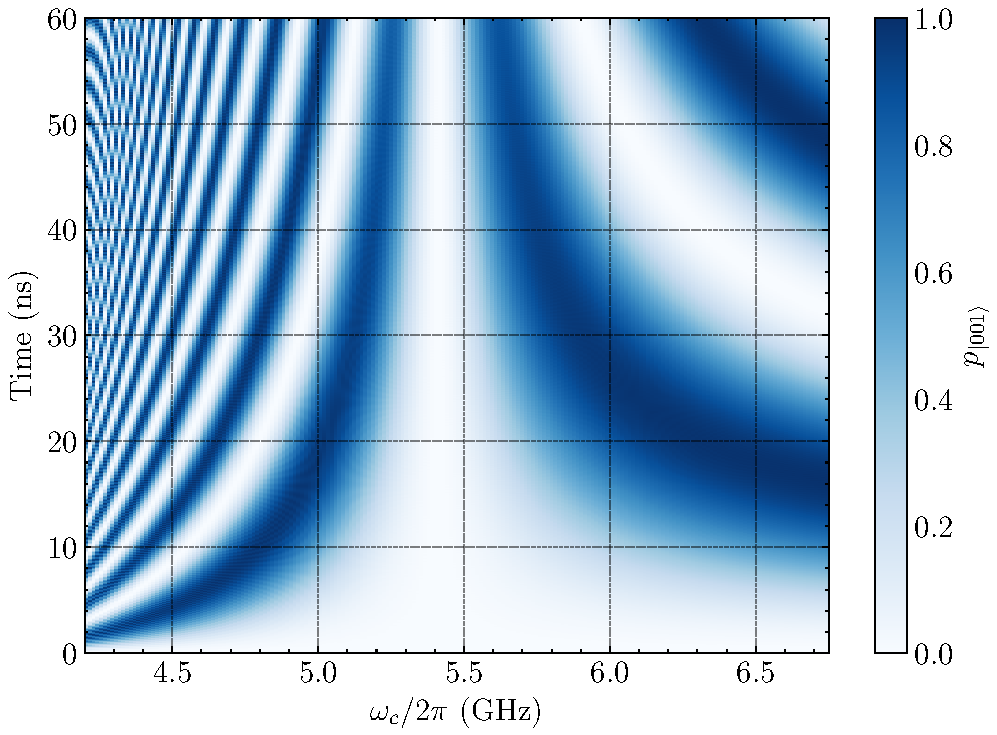
\includegraphics[width=.75\textwidth]{figures/TC_time_evolution.pdf}
    \caption{Time simulation results for the tunable coupler system in shown in Fig.\ \ref{fig:tc_circuit}. The system is initialized in state $\ket{100}$ and the two computational transmons are put on resonance such that $\omega_1/2\pi=\omega_2/2\pi=4$ GHz. The resulting oscillations in the population of state $\ket{001}$ are plotted above for various coupler frequencies.}
    \label{fig:tc_time_evolution}
\end{figure}

\begin{figure}[!h]
    \centering
    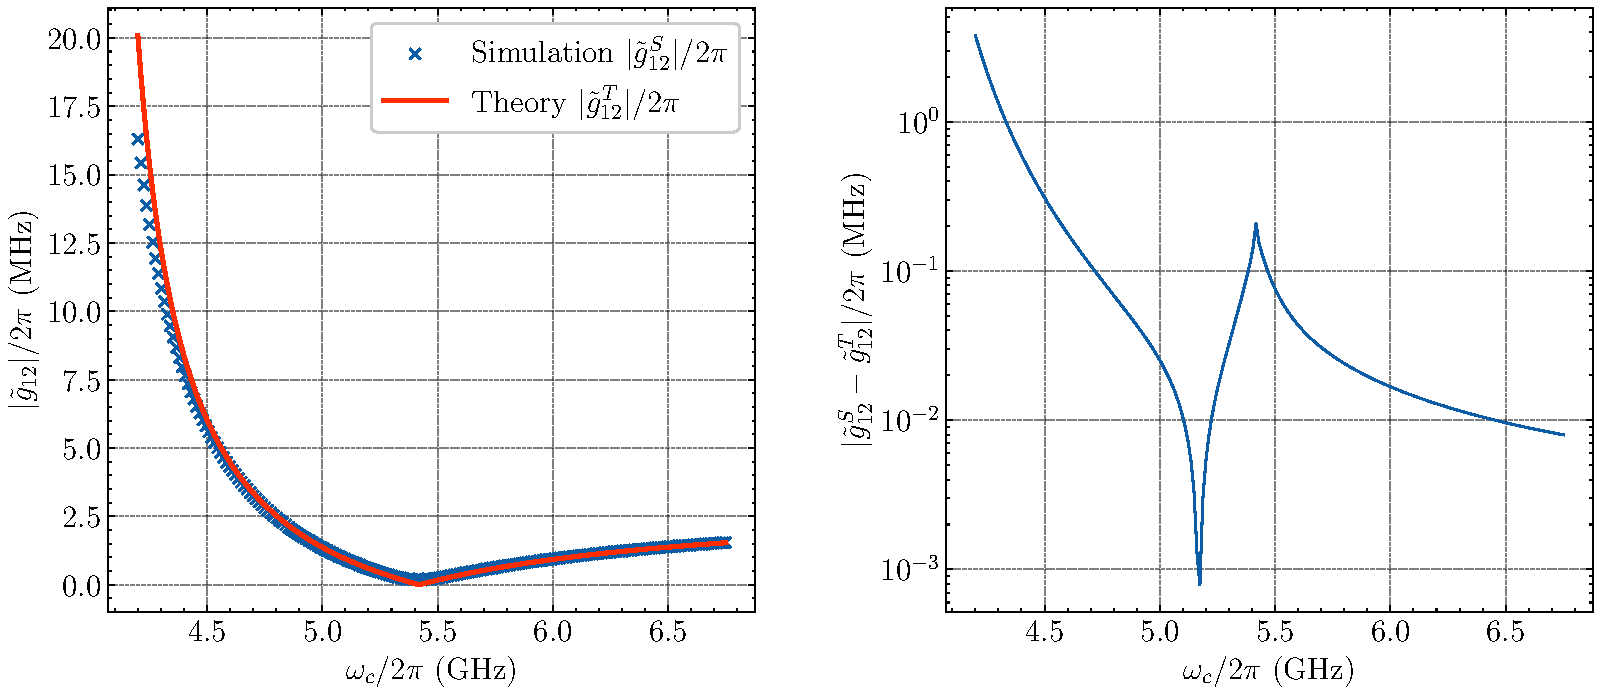
\includegraphics[width=\textwidth]{figures/TC_sim_th_eff_coupling.pdf}
    \caption{Left: Comparison between the theoretical and fitted effective coupling from the simulation in Fig.\ \ref{fig:tc_time_evolution}. Right: Difference between the theoretical and effective coupling extracted from the simulation.}
    \label{fig:eff_vs_sim_coupling}
\end{figure}

When attempting to implement fast two qubit gates in the nondispersive regime, leakage into the coupler can occur due to its higher participation in the coupling compared to the dispersive regime. An example of this is shown in Fig.\ \ref{fig:tc_time_evolve_example}. Nonetheless, the potential leakage to the coupler and higher energy levels during gate operations can be suppressed by control pulse optimization, which allows for fast gates to be implemented \cite{high_fidelity_cz_iswap_tc}. However, as we've seen, the formulas for the effective coupling rates (\ref{eq:eff_qubit_coupling}) will not be accurate in this regime. While not accurate in the nondispersive regime, the formulas can still provide a good estimate for the point at which the effective coupling is ``off''.

\begin{figure}[!h]
    \centering
    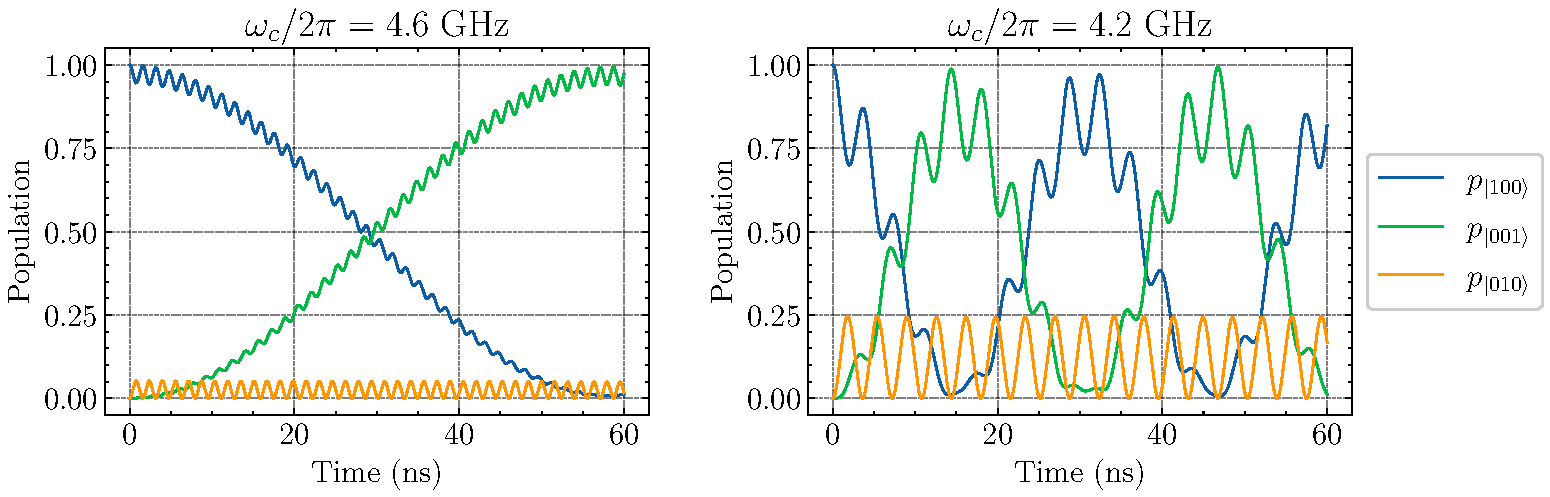
\includegraphics[width=\textwidth]{figures/TC_time_evolution_examples.pdf}
    \caption{Time evolution of state populations for circuit \ref{fig:tc_circuit} and $\omega_1/2\pi=\omega_2/2\pi=4$ GHz and two different coupler frequencies. On the left, for the higher coupler frequency, $g_{1c}/\Delta_{1c} \approx -0.12$. On the right, we have $g_{1c}/\Delta_{1c} \approx -0.345$.}
    \label{fig:tc_time_evolve_example}
\end{figure}


\subsection{Qubit Decay Rates}\label{section:decay_rate_example}
We will now see how the results of Section \ref{section:ext_ports_decay} can be applied to a lumped element circuit containing two coupled qubits and four external ports. We will also use the example circuit to demonstrate that (\ref{eq:qubit_decay_admittance}) can provide a good approximation to the qubit decay rates.

\begin{figure}[h!]
    \centering
    \begin{circuitikz}[line width=1pt]
        \normalfont
        \ctikzset{bipoles/thickness=1, bipoles/length=.75cm, monopoles/ground/thickness=0.65}
        \ctikzset { label/align = straight }

        % -------------------------------- Transmon 1 -------------------------------- %
        \draw (-2.8,0) to[C,l_=$C_{J_1}$] (-2.8,-1);
        \draw[color=nodecolor] (-2.2,0) to[barrier=$E_{J_1}$, label distance=-10pt] (-2.2,-1);

        % -------------------------------- Transmon 2 -------------------------------- %
        \draw (2.2,0) to[C,l_=$C_{J_2}$] (2.2,-1);
        \draw[color=nodecolor] (2.8,0) to[barrier=$E_{J_2}$, label distance=-10pt] (2.8,-1);

        % ------------------------ Top and bottom lines across ----------------------- %
        \draw (0,0) -- (0.75,0) to[C=$C_r$] (1.75,0) -- (3.25,0) to[C=$C_r$] (4.25,0) -- (5.75,0) to[C=$C_{r}$] (6.75,0) to[short, -o] (8,0);
        \draw (-8,0) to[short, o-] (-6.75,0) to[C=$C_{r}$] (-5.75,0) -- (-4.25,0) to[C=$C_r$] (-3.25,0) -- (-1.75,0) to[C=$C_r$] (-0.75,0) -- (0,0);
        \draw (-8,-1) to[short, o-] (0,-1) to[short,-o] (8,-1);
        \draw (0,-1) -- (-0,-1.05) node[ground] {};

        % ---------------------------------- Coupler --------------------------------- %
        \draw (-0.3,0) to[C,l_=$C_c$] (-0.3,-1);
        \draw (0.3,0) to[L=$L_c$] (0.3,-1);

        % ----------------------- Transmon 1 Readout Resonator ----------------------- %
        \draw (-5.3,0) to[C,l_=$C_c$] (-5.3,-1);
        \draw (-4.7,0) to[L=$L_{R_1}$] (-4.7,-1);

        % ----------------------- Transmon 2 Readout Resonator ----------------------- %
        \draw (4.7,0) to[C,l_=$C_c$] (4.7,-1);
        \draw (5.3,0) to[L=$L_{R_2}$] (5.3,-1);

        % ----------------------- Readout Port Shunt Capacitors ---------------------- %
        \draw (-7.25,0) to[C=$C_s$] (-7.25,-1);
        \draw (7.25,0) to[C,l_=$C_s$] (7.25,-1);

        % -------------------------------- Drive Ports ------------------------------- %
        \draw (-2.5,0) -- (-2.5,2) to[C,l_=$C_d$] (-4.5,2) to[short, -o] (-5.5,2);
        \draw (-4.5,2) to[C=$C_s$] (-4.5,1) to[short,-o] (-5.5,1);
        \draw (-4.5,1) -- (-4.5,.95) node[ground] {};

        \draw (2.5,0) -- (2.5,2) to[C,l=$C_d$] (4.5,2) to[short, -o] (5.5,2);
        \draw (4.5,2) to[C,l_=$C_s$] (4.5,1) to[short,-o] (5.5,1);
        \draw (4.5,1) -- (4.5,.95) node[ground] {};

    \end{circuitikz}
    \caption{Circuit model for two resonator-coupled transmons where each is individually coupled to an external drive port and readout resonator. Overall, there are four external ports, two for drive, and two for readout. When discussing this circuit, we sometimes refer to the two transmon or qubit ports that are located at the positions of the Josephson junctions (marked in red). Transmons 1 and 2 have the Josephson energies $E_{J_1}$ and $E_{J_2}$, respectively. The values of the circuit elements are as follows: $C_{J_1}=$ 70 fF, $C_{J_1}=$ 75 fF, $C_s=$ 100 fF, $C_c=$ 300 fF, $C_r=$ 10 fF, $C_d=$ 0.15 fF, $L_c=$ 3.25 nH, $L_{R_1}=$ 2.1 nH, and $L_{R_2}=$ 1.6 nH. The external ports are assumed to have characteristic impedances of $Z_0=$ 50 $\Omega$.}
    \label{fig:decay_lumped_circuit}
\end{figure}

We consider the circuit in Fig. \ref{fig:decay_lumped_circuit}. If we fix the qubit inductances, we can find the eigenvalues of the matrix in (\ref{eq:matrix_eoms}) to obtain the complex poles that correspond to the resonant modes in the circuit. From these eigenvalues, we find two complex conjugate pairs that correspond to the transmon oscillator modes. Three other complex conjugate pairs are also found for the other resonant modes in the circuit. Now, we want to verify that these complex numbers are the complex poles of the impedance function for the circuit in Fig.\ \ref{fig:decay_lumped_circuit} with the external ports shunted by resistors and the transmon ports shunted by inductors (as shown in Fig.\ \ref{fig:lossy_transmon_network}). To compute the shunted impedance function at an arbitrary complex frequency, we first compute the impedance function for the circuit Fig.\ \ref{fig:decay_lumped_circuit} using the method of Section \ref{section:cascade_analysis}. Then we shunt the qubit ports with inductors and the external ports with resistors using (\ref{eq:cascade_s}). We find that the predicted pole locations from (\ref{eq:matrix_eoms}) match the positions of the poles of the lossy impedance function. This alignment is shown for one of the transmon poles in Fig.\ \ref{fig:shunted_impedance_plot}.

\begin{figure}[!h]
    \centering
    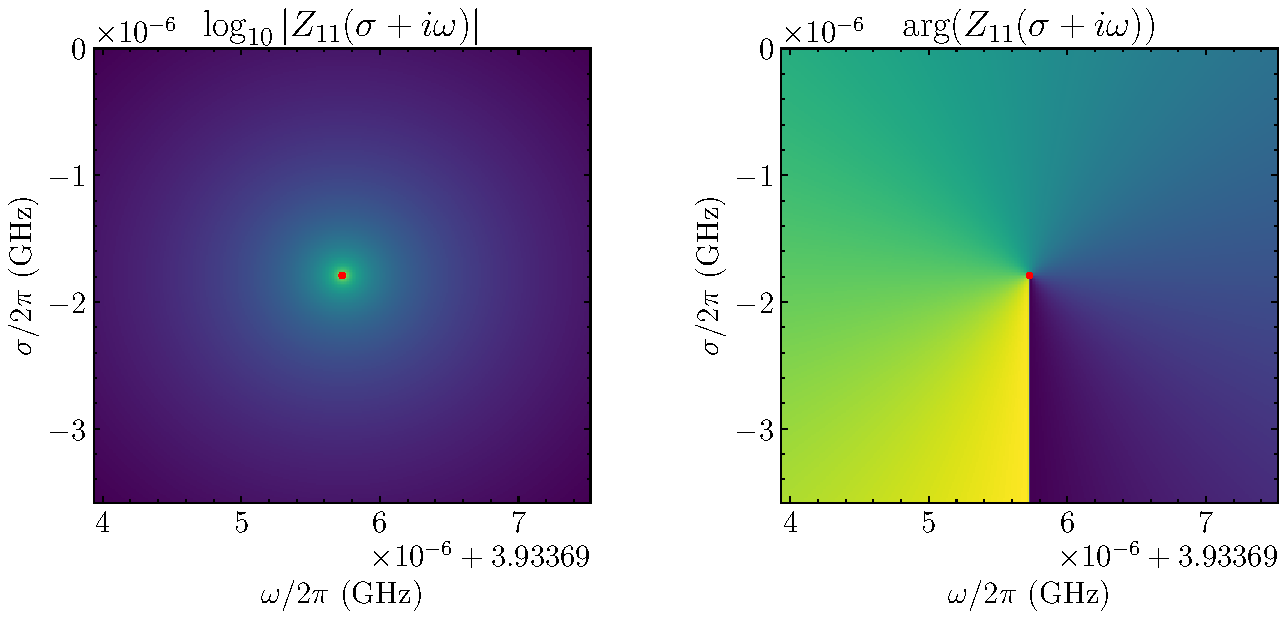
\includegraphics[width=\textwidth]{figures/fully_shunted_impedance.pdf}
    \caption{These plots show the magnitude and phase of the impedance function for the circuit in Fig.\ \ref{fig:decay_lumped_circuit} with inductors and resistors shunting the transmon and external ports, respectively. We have chosen $L_{J_1}=$ 18 nH and $L_{J_2}=$ 15.5 nH. In the plot, we look at a region around a complex pole that corresponds to transmon 1 in the circuit. We find that the predicted pole position computed by diagonalizing (\ref{eq:matrix_eoms}) aligns with the pole position in the numerically computed impedance.}
    \label{fig:shunted_impedance_plot}
\end{figure}

We have shown that diagonalizing (\ref{eq:matrix_eoms}) does in fact provide us with the complex poles of the shunted impedance function for a network of the form shown in Fig.\ \ref{fig:lossy_transmon_network}. With the complex pole positions, we can estimate the decay rate for a given resonant frequency using (\ref{eq:lossy_pole}). We can use this to compute the decay rates of the transmons at various frequencies by varying one of the transmon inductances and computing the poles for each inductance value. As an example, we do this for transmon 1 in the circuit, and the decay rates and resonant modes for all the computed poles are plotted in Fig.\ \ref{fig:poles_real_imag}. In these plots, we can see how the resonance frequency and decay rate of the transmon oscillator changes as the shunt inductance is changed.

Taking this method further, we can then see the relationship between the transmon resonant frequency and its relaxation time $T_1 = \kappa^{-1}$. We compare this to the qubit decay rate estimate using the admittance of the lossy network (\ref{eq:qubit_decay_admittance}). For the admittance, we can also choose to include or exclude the transmon inductances. We do this for both qubits and the results of the three methods are shown in Fig.\ \ref{fig:transmons_T1}. When plotting the poles computed from (\ref{eq:matrix_eoms}), there are peaks in the transmon lifetimes that are present due to the avoided level crossings shown in Fig.\ \ref{fig:poles_real_imag}. At the resonance crossings, the transmon oscillator is not well defined on its own, and thus the peaks should not be thought of as an expected point where the transmon lifetime is increased. In the plot using the admittance with ports shunted by inductors and resistors, there are sharp dips present that are not seen when only shunting with resistors. These dips are present because of the additional resonance mode of the other transmon. Comparing the methods, we see that using the admittance estimates can provide a good lower bound on the transmon relaxation times. We can also show that if we increase the coupling complexity of the network, this is still the case. We show this by adding a 1 fF capacitance between every node where one is not already present for the circuit in Fig.\ \ref{fig:decay_lumped_circuit}. The results for the relaxation time estimates for this new network are shown in Fig.\ \ref{fig:transmons_T1_ata}.

\begin{figure}[!h]
    \centering
    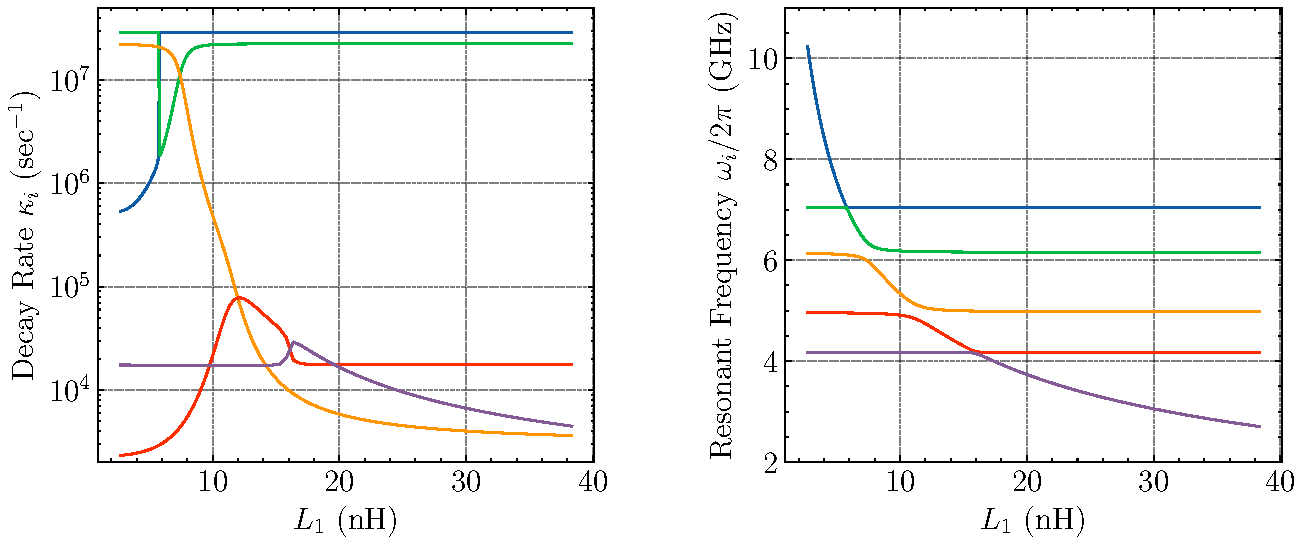
\includegraphics[width=\textwidth]{figures/poles_real_imag.pdf}
    \caption{Decay rates and resonant frequencies of the complex poles found by diagonalizing the matrix in (\ref{eq:matrix_eoms}) while varying the inductance shunting transmon 1. The inductance of transmon 2 is fixed at $L_{J_2}=$ 13.8 nH.}
    \label{fig:poles_real_imag}
\end{figure}

\begin{figure}[!h]
    \centering
    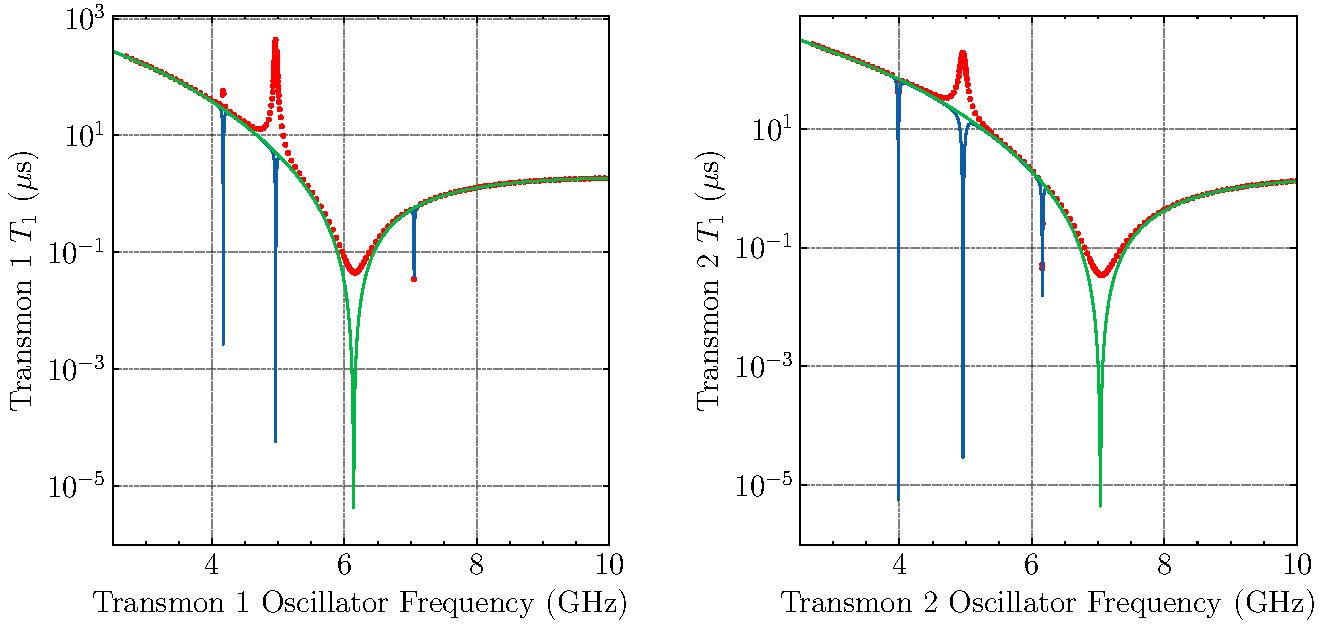
\includegraphics[width=\textwidth]{figures/lumped_transmons_T1.pdf}
    \caption{Above, we use three methods to plot estimates of the $T_1$ time of transmons 1 and 2 for the circuit in Fig.\ \ref{fig:decay_lumped_circuit}. \textbf{Red points:} The positions of the complex poles of the network found by diagonalizing the matrix in (\ref{eq:matrix_eoms}). As one transmon inductance is varied, the other is fixed. In the left plot, $L_{J_2}=$ 15.2 nH and on the right, $L_{J_1} =$ 17.5 nH. \textbf{Blue line:} $\Gamma_i^{-1}$ computed using the admittance in (\ref{eq:qubit_decay_admittance}) with the transmon ports shunted with inductors and the external ports shunted with resistors. \textbf{Green line:} Also using (\ref{eq:qubit_decay_admittance}), but the admittance is only shunted with resistors at the external ports.}
    \label{fig:transmons_T1}
\end{figure}

\clearpage
\begin{figure}[!h]
    \centering
    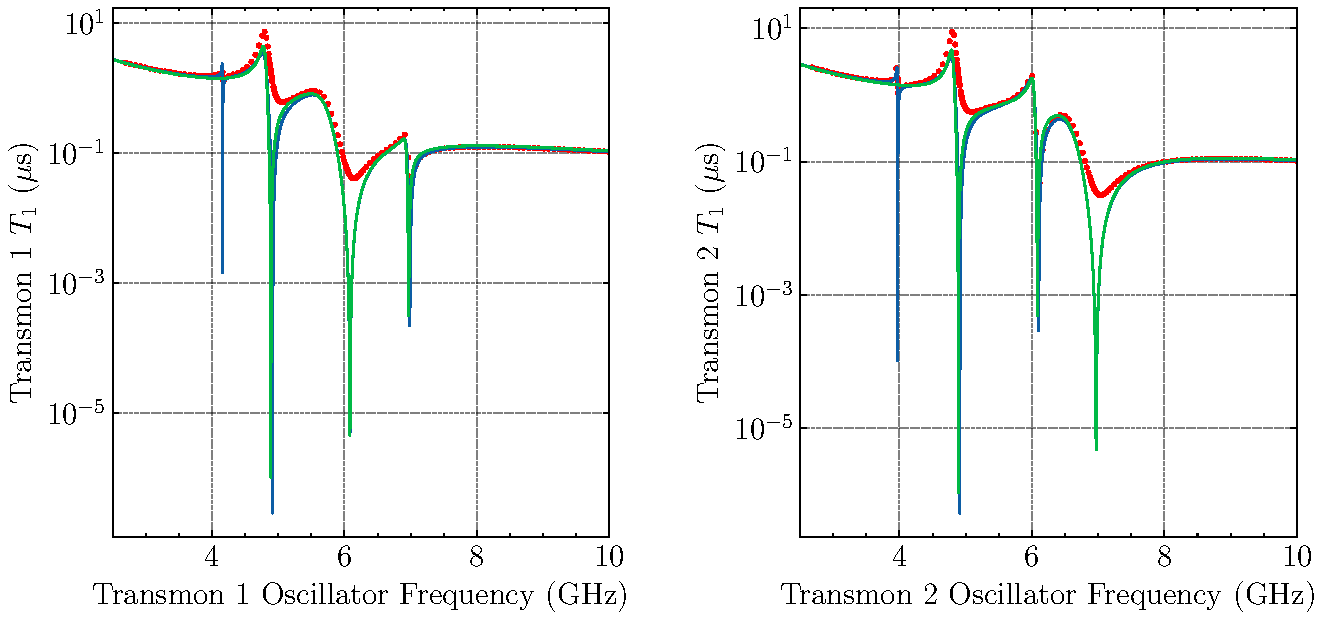
\includegraphics[width=\textwidth]{figures/lumped_transmons_T1_all_to_all.pdf}
    \caption{Same as Fig.\ \ref{fig:transmons_T1} except now there is an added 1 fF capacitance between nodes where there was no coupling present for the circuit in Fig.\ \ref{fig:decay_lumped_circuit}.}
    \label{fig:transmons_T1_ata}
\end{figure}

\subsection{Ideal Transmission Line Coupler}
Here, we consider a network of two qubits coupled by an ideal transmission line as shown in Fig.\ \ref{fig:ideal_TL_coupler}. Now we go through the process of obtaining the Hamiltonian from the impedance function of this two-port network.

\begin{figure}[h!]
    \centering
    \begin{circuitikz}[line width=1pt]
    \ctikzset{american}
    \ctikzset{bipoles/thickness=1, bipoles/length=1cm}
    \ctikzset{bipoles/crossing/size=0.5}
    \ctikzset { label/align = straight }

    \draw[color=nodecolor] (-2.5,1) -- (-3,1) to[barrier=$E_{J_1}$, label distance=-10pt]  (-3,-0.5) -- (-2.5,-0.5);
    \draw[color=nodecolor] (11,1) -- (11.5,1) to[barrier,l_=$E_{J_2}$, label distance=-10pt]  (11.5,-0.5) -- (11,-0.5);
    
    \draw (-2.5,1) to[short,o-] (0,1) to[short, o-] (0.5,1) to[C=$C_{1c}$] (2,1) to[short, -o] (2.5,1) to[short,-o] (6,1) -- (6.5,1) to[C=$C_{2c}$] (8,1) to[short, -o] (8.5,1) to[short, -o] (11,1);
    \draw (-2.5,-0.5) to[short,o-] (0,-.5) to[short,o-] (0.5,-.5) to[short, -o] (2.5,-.5) to[short, -o] (6,-.5) to[short,-o] (8.5,-.5) to[short, -o] (11,-0.5);

    \draw (-1.25,1) to[C=$C_1$] (-1.25,-0.5);
    \draw (9.75,1) to[C,l_=$C_2$] (9.75,-0.5);
    

    \node at (4.25,0.25) {$Z_0,\; \beta=\omega\sqrt{LC}$};
    
    \node at (4.25,-0.75) {$\ell$};
    \draw [-stealth](4.5,-0.75) -- (6,-0.75);
    \draw [-stealth](4,-0.75) -- (2.5,-0.75);

    \end{circuitikz}
    \caption{Two qubit circuit containing two transmon qubits coupled by an ideal transmission line. The network can be viewed as a two-port system shunted with two Josephson junctions.}
    \label{fig:ideal_TL_coupler}
\end{figure}

We can compute the two-port impedance function over a discretized frequency range by using ABCD matrices \cite[Chapter 4.4]{Pozar_2011}. The network in Fig.\ \ref{fig:ideal_TL_coupler} is broken up into pieces containing either a capacitor or the transmission line where each has a simple ABCD matrix representation. Then, we cascade all of the ABCD matrices and convert to an two-port impedance function that is discretized in frequency. The next step is to obtain the rational impedance function that approximates the response of this network. We do this by using the vector fitting methods as described in Section \ref{section:vector_fitting}. For this circuit, taking the lossless part of the rational model obtained from the traditional vector fitting process already produces a good approximation with the results shown in Fig.\ \ref{fig:ideal_TL_coupler_fit}. For this example, we fit for a frequency range of 1 GHz to 22.5 GHz. The final fitted rational function of the form (\ref{eq:impedance}) has four resonant poles that are clearly seen in the frequency range. We could also try to fit for the next highest resonant pole that is ``invisible'' to the fitting process. Generally when doing the fitting, poles within the frequency range chosen can be restricted to be nondegenerate. Outside the frequency range, degenerate poles may appear and they may also not be where you expect (e.g. at the next highest mode of one of the resonators). For this case, we don't try to fit these poles since we want to avoid adding incorrect resonant modes to this model. 

\begin{figure}[!h]
    \centering
    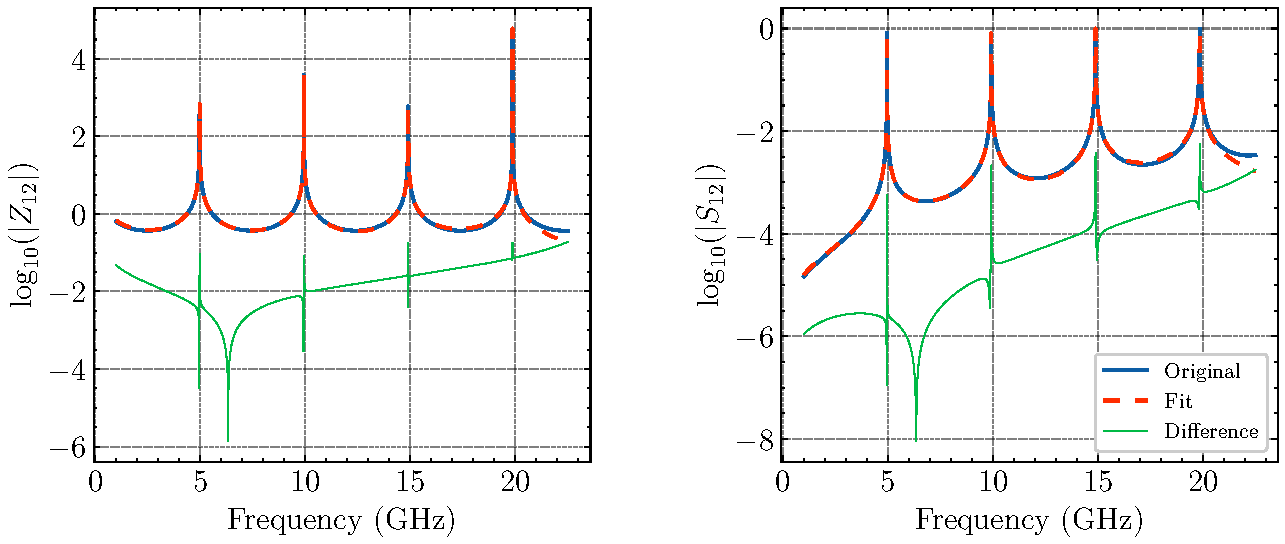
\includegraphics[width=\textwidth]{figures/ideal_TL_fit.pdf}
    \caption{Fit results for the off-diagonal elements of the impedance and scattering parameters for the two-port network in Fig.\ \ref{fig:ideal_TL_coupler}. The diagonal elements of the parameters show similar or smaller difference. For the capacitors we choose $C_1 =$ 70 fF, $C_2 =$ 72 fF, $C_{1c}=C_{2c} =$ 6.5 fF. For the transmission line we choose $L = $ 0.438 $\mu$H/m, $C = $ 0.159 nF/m, $\ell =$ 12 mm.}
    \label{fig:ideal_TL_coupler_fit}
\end{figure}

Using the fitted rational impedance function, we can write out the Hamiltonian of the system using (\ref{eq:impedance_hamiltonian}) once we've taken into account the Josephson junctions at the ports. With both transmons at $\omega_1/2\pi=\omega_2/2\pi = $ 4 GHz, they have a direct coupling rate of $g_{12} = 0.652$ MHz. The coupling rates of the transmons to the resonant modes are shown in Table \ref{table:ideal_TL_coupling}.

\renewcommand{\arraystretch}{1.5}
\begin{table}[h!]
    \centering
    \begin{tabular}{|r|r|r|r|r|}
    \hline
    $\omega_{R_k}/2\pi$ (GHz) & $4.965470$   & $9.931947$   & $14.896434$  & $19.8619404$ \\ \hline
    $g_{1,R_k}/2\pi$ (MHz)   & $-55.113$ & $-77.924$ & $-95.422$ & $-110.154$ \\ \hline
    $g_{2,R_k}/2\pi$ (MHz)   & $54.367$  & $-76.869$ & $94.130$  & $-108.662$ \\ \hline
\end{tabular}
\caption{The resonant pole positions $\omega_{R_k}$ from the fit result in Fig.\ \ref{fig:ideal_TL_coupler_fit} and their corresponding coupling rates to the transmons.}
\label{table:ideal_TL_coupling}
\end{table}
\renewcommand{\arraystretch}{1}

Using the resulting Hamiltonian, we can construct the effective Hamiltonian for the system that only contains the transmons. Then we can simulate the time evolution of the full Hamiltonian (\ref{eq:transmon_resonator_ham}) containing the four resonant modes and compare it to the simulation of the effective Hamiltonian (\ref{eq:eff_ham}). An example showing agreement between the two is shown in Fig.\ \ref{fig:ideal_TL_coupler_sim}.

\begin{figure}[!h]
    \centering
    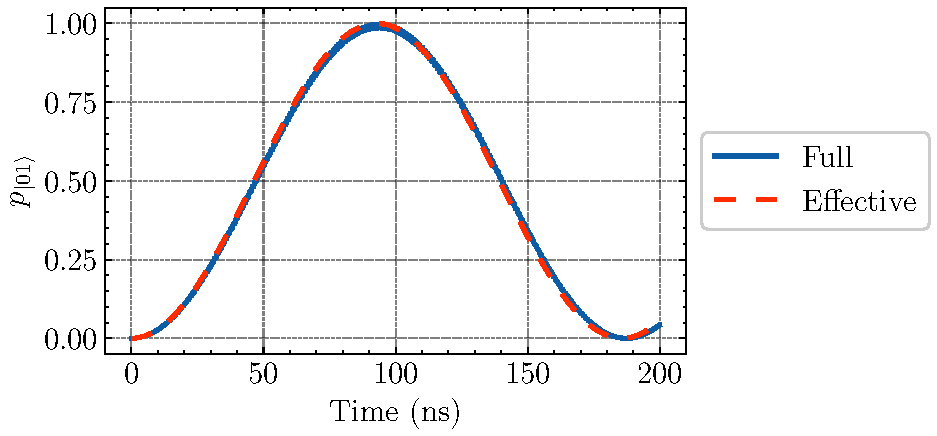
\includegraphics[width=0.6\textwidth]{figures/ideal_TL_sim.pdf}
    \caption{Time evolution of the full and effective Hamiltonians for the circuit in Fig.\ \ref{fig:ideal_TL_coupler} using the results from the fit in Fig.\ \ref{fig:ideal_TL_coupler_fit}. The transmons are at 4 GHz and the initial state is $\ket{Q_1Q_2}=\ket{10}$ with all the resonators of the full Hamiltonian in the ground state.}
    \label{fig:ideal_TL_coupler_sim}
\end{figure}

Using the same circuit, we can look at what happens to our estimate of the effective coupling rate between the qubits when we increase the cutoff frequency used for our fit. When increasing this range, more resonances are visible in the response and are then included as new resonance modes in the fitted rational impedance. We start by fitting a function that includes just the first resonant mode. Then for each of the next highest resonant modes, we fit new functions until we have reached a total of 40 resonant modes included. Note that this is only performed as a test of the fitting process and to see how the effective coupling formulas are affected by including these higher resonant modes. The fit for the frequency range that contains 40 resonant modes is shown in Fig.\ \ref{fig:ideal_TL_coupler_fit_40_res}. The fitting for this wide frequency range is quick (less than 30 seconds) and the results here only use the lossless part of the impedance obtained from the traditional vector fitting process.

\begin{figure}[!h]
    \centering
    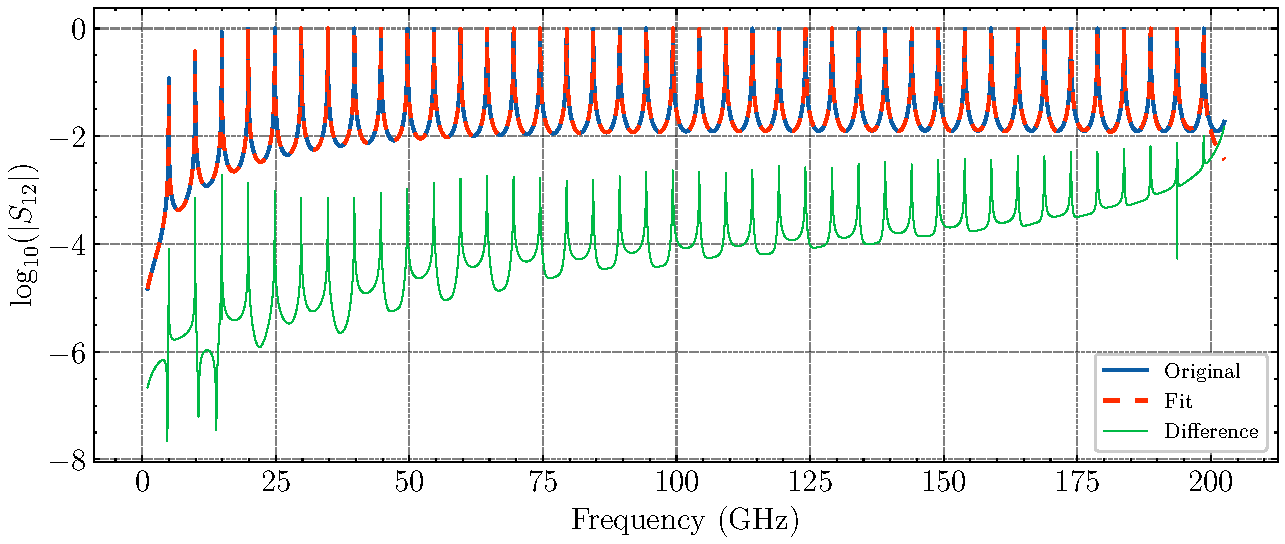
\includegraphics[width=\textwidth]{figures/ideal_TL_fit_40_res.pdf}
    \caption{Fit results for the $S_{12}$ parameter for the two-port network in Fig.\ \ref{fig:ideal_TL_coupler}. Here, 40 resonant modes are included in the frequency range.}
    \label{fig:ideal_TL_coupler_fit_40_res}
\end{figure}

\begin{figure}[!h]
    \centering
    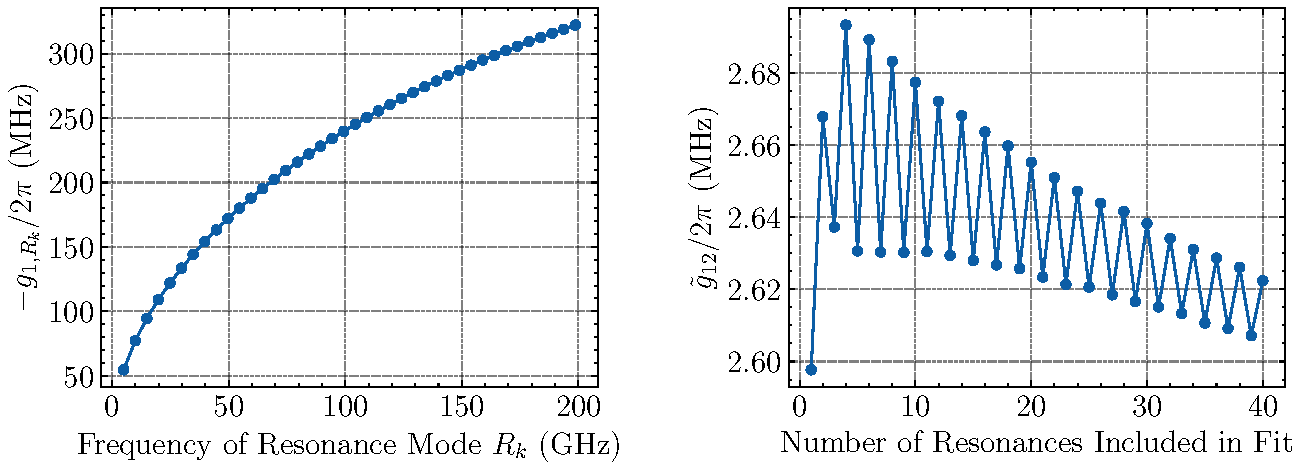
\includegraphics[width=\textwidth]{figures/ideal_TL_coupling_change.pdf}
    \caption{Left: For the fitted network in Fig.\ \ref{fig:ideal_TL_coupler_fit_40_res}, the coupling $g_{1,R_k}$ is shown for all 40 resonant modes present in the fit. Right: Effective coupling estimate (\ref{eq:eff_qubit_coupling}) as a function of the number of resonances included in the fit of the impedance function. Transmon frequencies are $\omega_1/2\pi=\omega_2/2\pi = $ 4 GHz.}
    \label{fig:ideal_TL_geff_change}
\end{figure}

First, we see that the coupling between the resonant modes and the transmons diverge as the resonant modes goes to higher frequency ($g_{i,R_k} \propto \omega_{R_k}^{1/2}$). This divergence is expected given that the Hamiltonian (\ref{eq:transmon_hamiltonian}) that we start with cannot account for the infinite number of resonant modes introduced by the ideal transmission line \cite{Parra-Rodriguez_2018}. This has the effect that the estimate of the effective coupling will also diverge if continuing to include higher resonant modes. In the effective coupling there is also an oscillation due to the alternating signs present in the coupling of one of the transmons to the resonant modes. This can be seen clearly in Table \ref{table:ideal_TL_coupling} and also in a similar example in Appendix \ref{appendix:cascade_ideal_TL}. In reality, there is a natural cutoff frequency for these resonant modes that is dependent on the superconducting gap frequency. In addition, there will be higher loss or attenuation in the material at higher frequencies that will reduce the coupling through the higher resonant modes \cite{picosecond_pulses,harmonic_superconducting}. These factors can help in choosing the cutoff frequency for our fitting.
\section{Electromagnetic Models}

In this section, we explore how the vector fitting and interconnection methods can be used for characterizing electromagnetic models of superconducting circuits. To obtain the multiport impedance parameters needed for our characterization methods, we use Ansys HFSS \cite{ansys_hfss} for the full-wave FEM electromagnetic simulations and Qiskit Metal \cite{Qiskit_Metal} for some of the device modeling. Also, when working with some of the simulation results we have used the Python package scikit-rf \cite{scikit_rf}.

\subsection{Brick Building Approach}

Simulating a full electromagnetic model of a multi-qubit superconducting circuit can be prohibitively expensive if trying to obtain the impedance parameter over a broad frequency range. To tackle this, we propose a method where circuit designs can be broken up into smaller and simpler ``bricks". Then, these pieces can be interconnected to obtain a model of a larger device. Since the number of ports and resonant modes for each of these bricks will be much smaller than for the full model, applying the fitting methods of Section \ref{section:vector_fitting} is possible. If we have the rational impedances of multiple bricks, we can then use the method of Section \ref{section:rational_impedance_interconnection} to obtain the rational impedance function of the larger interconnected model. From this rational impedance function, we can easily construct a circuit Hamiltonian.

Splitting up your circuit does not come without compromise. For example, capacitive coupling between qubits in different bricks will not be taken into account accurately. However, since we obtain the full Hamiltonian of the system, any potential cross-brick coupling that is not taken into account can be added in afterwards. For this, we would need to estimate the long range capacitive coupling of the components in the circuit, which can be done using formulas for planar electrodes \cite{planar_capacitance} or potentially with simpler capacitance only simulations.

To see an example of the brick building method in action, we look at how it can be applied to the model in Fig.\ \ref{fig:cap_res_cap_full}. The circuit in Fig.\ \ref{fig:cap_res_cap_full} is a two port network which contains a half-wave coplanar waveguide (CPW) resonator that is capacitively coupled to the two ports. In this simulation and the ones that follow, the models will contain perfectly conducting sheets on top of a silicon substrate. Sometimes, wirebonds are also included over meandered CPWs. Wave ports are used for the ports located at the boundary of the model. We will compare the simulation results of this model to the split model as shown in Fig.\ \ref{fig:cap_res_cap_split}.

\begin{figure}[!h]
    \centering
    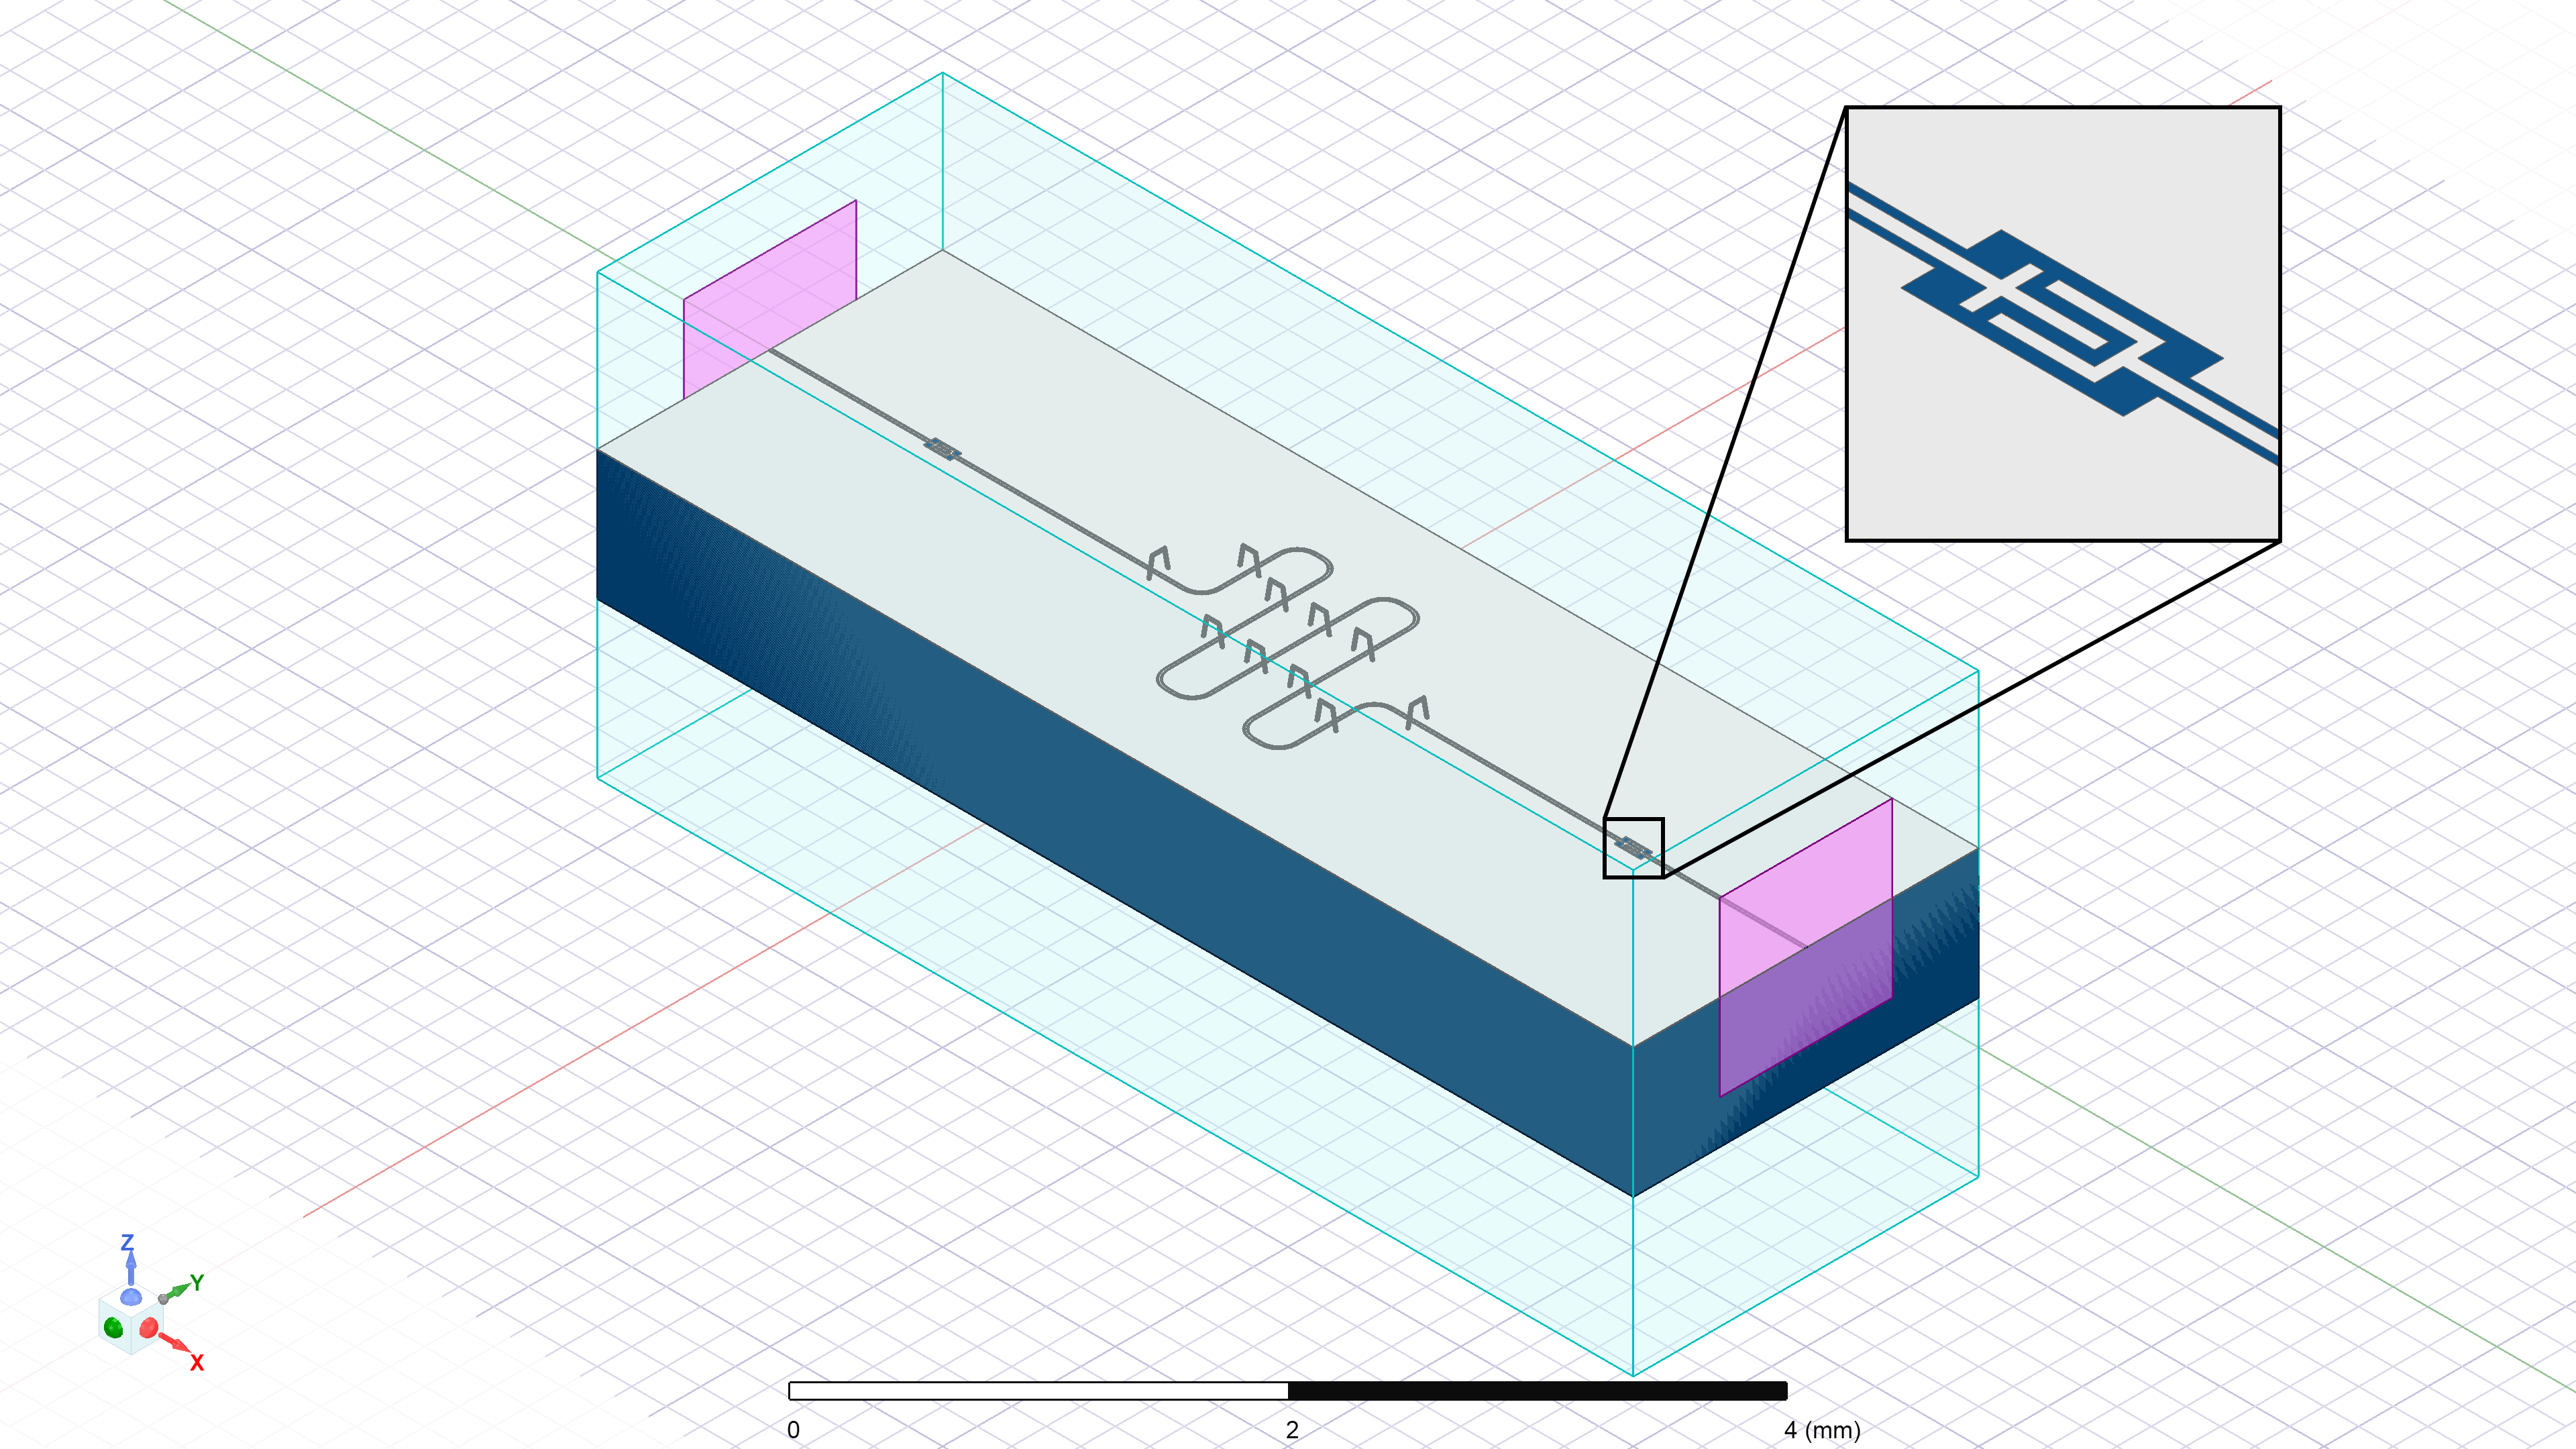
\includegraphics[width=\textwidth]{figures/cap_res_cap_full.png}
    \caption{Two port circuit containing an 8 mm half-wave CPW resonator that is capacitively coupled to the two external ports.}
    \label{fig:cap_res_cap_full}
\end{figure}

\begin{figure}[!h]
    \centering
    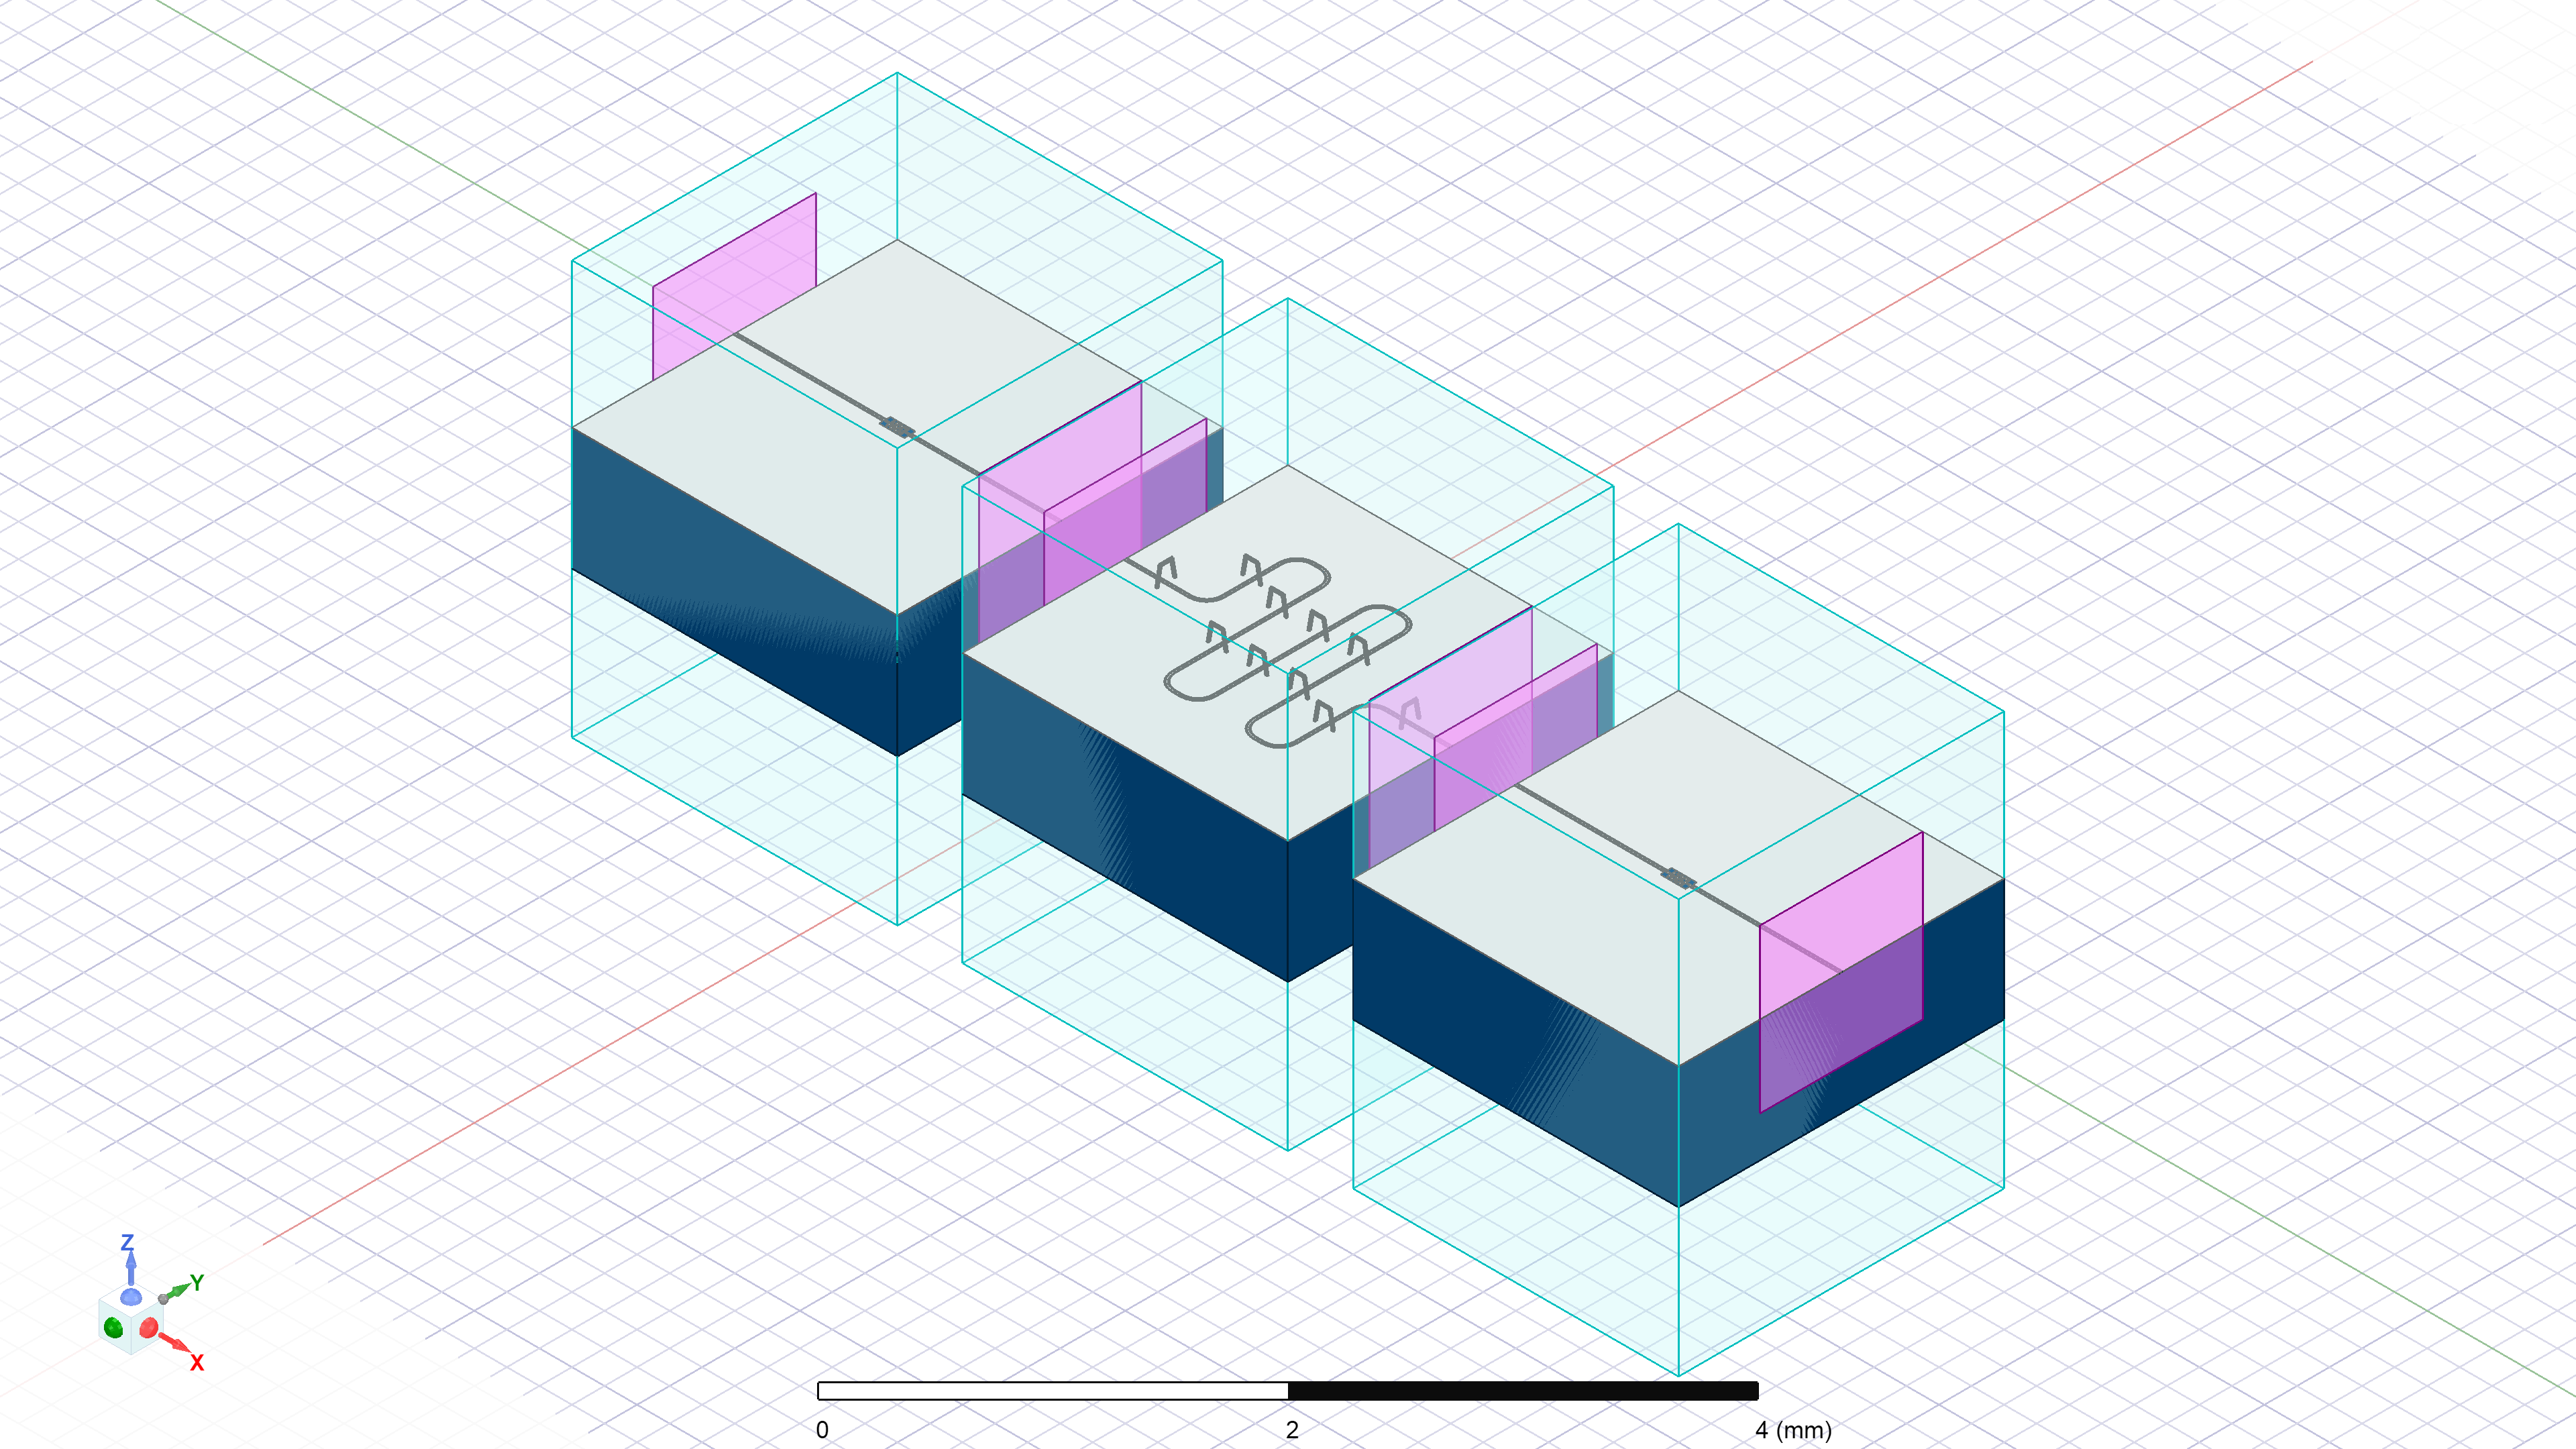
\includegraphics[width=\textwidth]{figures/cap_res_cap_split.png}
    \caption{Split version of the model in Fig.\ \ref{fig:cap_res_cap_full}. The left and right bricks are identical and only contain the finger capacitor coupled to the two ends with CPWs. The center brick only contains a 6 mm CPW.}
    \label{fig:cap_res_cap_split}
\end{figure}

For all of our simulations we will use the interpolating sweep options in HFSS, where the software chooses at what frequencies to solve the model, and then interpolates the solution with its own fitting methods. The model is repeatedly solved and fitted until the difference in S-parameters between runs is under a specified percentage. We have chosen an error tolerance of 0.5\% for these examples. Alternatively, we could pick these frequency points ourselves and apply the fitting methods directly. We are also using the adaptive fitting methods within HFSS to obtain a mesh that has a convergence at the high end of the our chosen frequency range (20.5 GHz). The mesh for the model in Fig.\ \ref{fig:cap_res_cap_full} is shown in Fig.\ \ref{fig:cap_res_cap_mesh}.

We then apply the fitting process from Section \ref{section:vector_fitting} to the simulations of the bricks in Fig.\ \ref{fig:cap_res_cap_split}. The results of the fitting are shown in Fig.\ \ref{fig:cap_res_fit}. Then, using the interconnection method of Section \ref{section:rational_impedance_interconnection}, we can stitch bricks together to obtain a final rational impedance function. To show the difference between the full model and the brick model, we compare the $S_{12}$ parameters in Fig.\ \ref{fig:full_vs_brick}. In this comparison, we see that primary differences are in the resonance frequencies of the full model and the brick model. We estimate that the resonance frequency of the fundamental mode in the brick model is approximately 15 MHz higher ($+0.2$\%) compared to the full model. We also confirm that this is not due to the fitting by comparing the interconnected model before and after the fit and finding a negligible difference. This suggests that the modeling of these bricks can be improved. One potential cause of the difference is the meshes for the full and split models. To improve on this, we could potentially decrease the error tolerance for the adaptive meshing process which in this case is at 1\%. We could also make the adaptive meshing process sample results from more frequency points. Another potential problem with the split model could be the dimensions of the wave ports. These points in addition to other components such as the interpolating sweeps and even comparison with other simulation software should be explored further in any implementations of this splitting method.

\begin{figure}[!t]
    \centering
    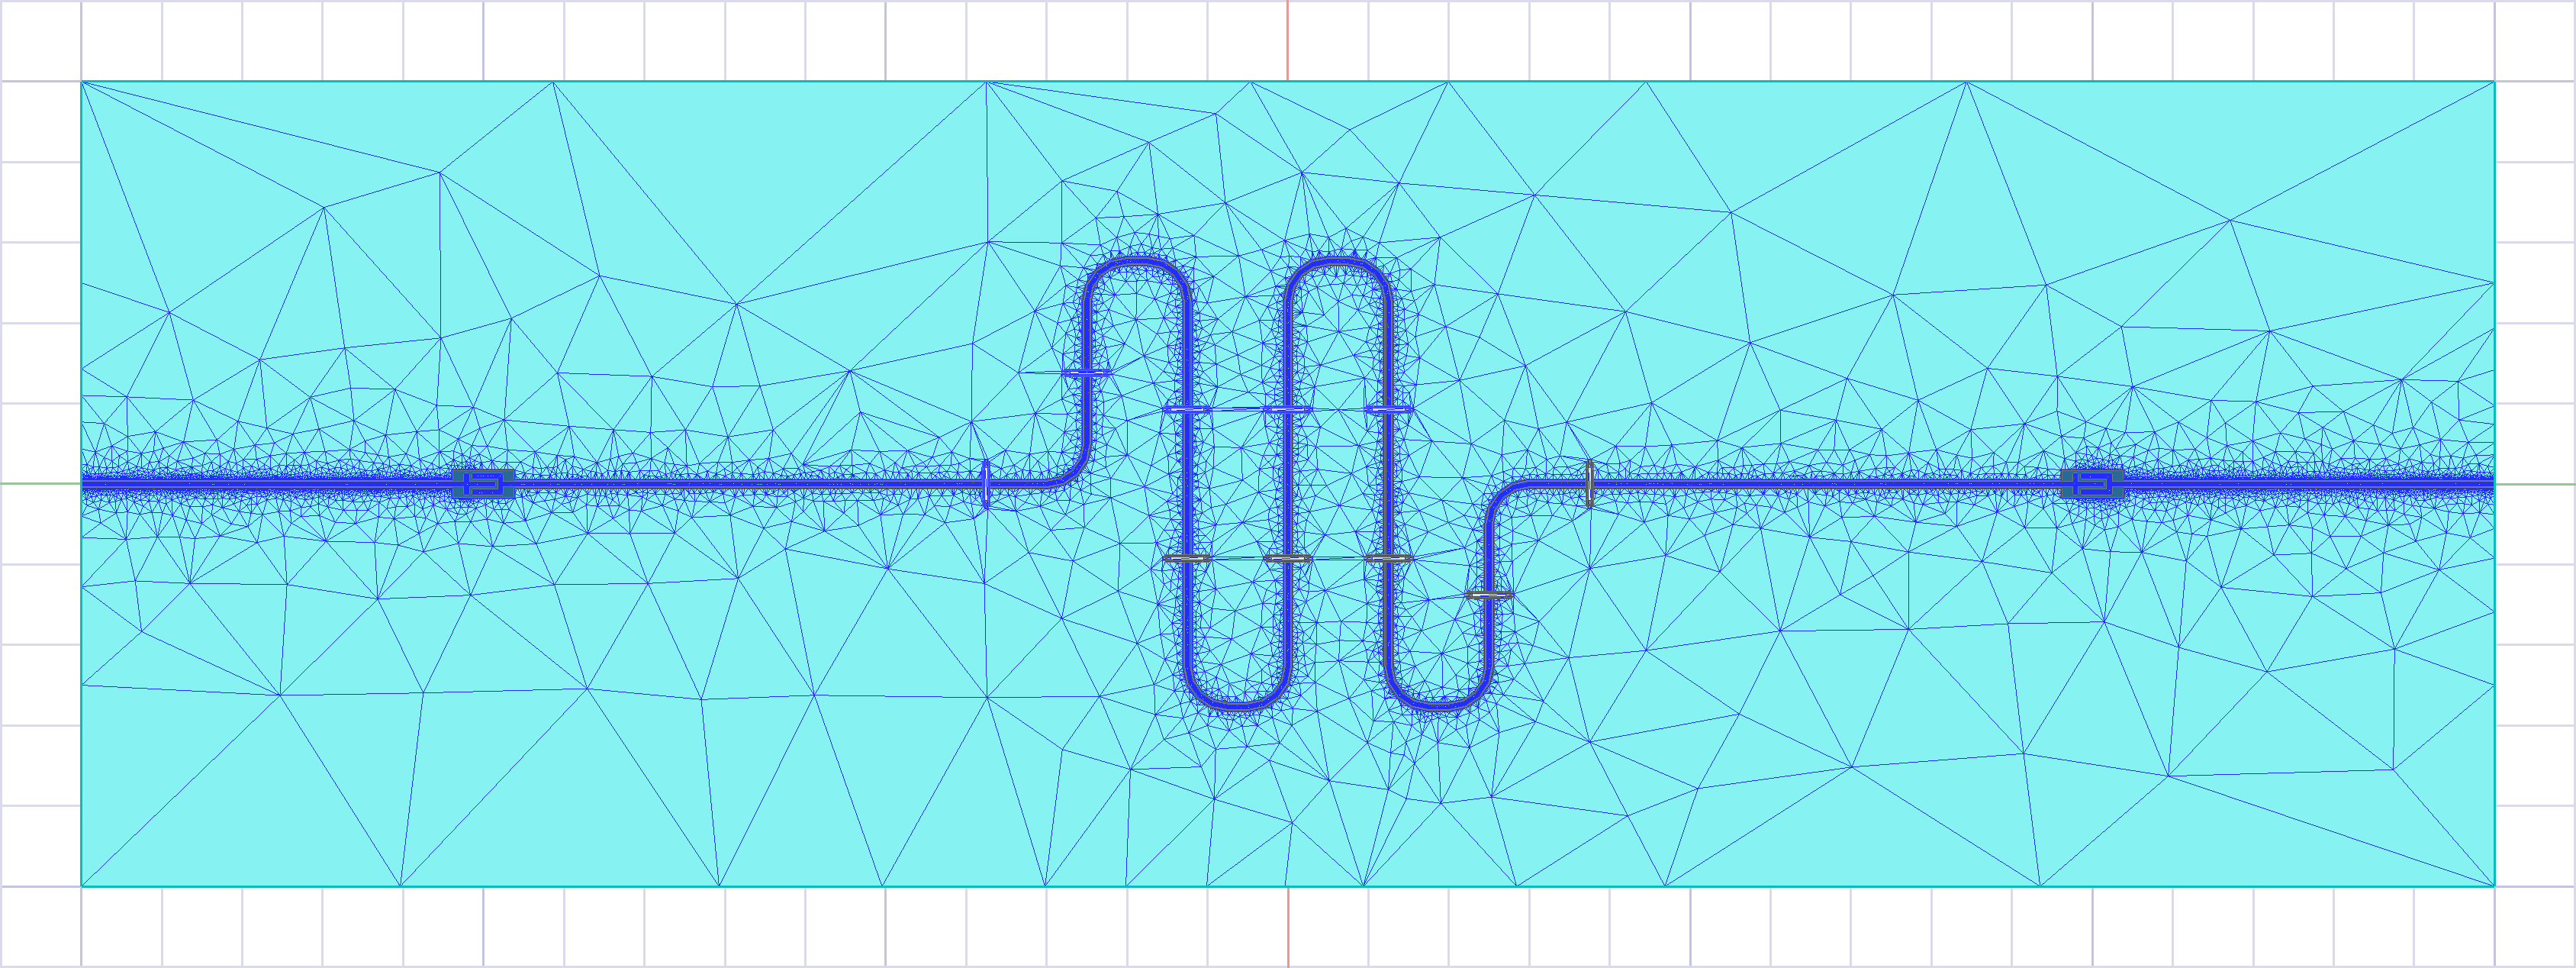
\includegraphics[width=\textwidth]{figures/cap_res_cap_mesh.png}
    \caption{Mesh used for the simulation of the model in Fig.\ \ref{fig:cap_res_cap_full}.}
    \label{fig:cap_res_cap_mesh}
\end{figure}

\begin{figure}[!t]
    \centering
    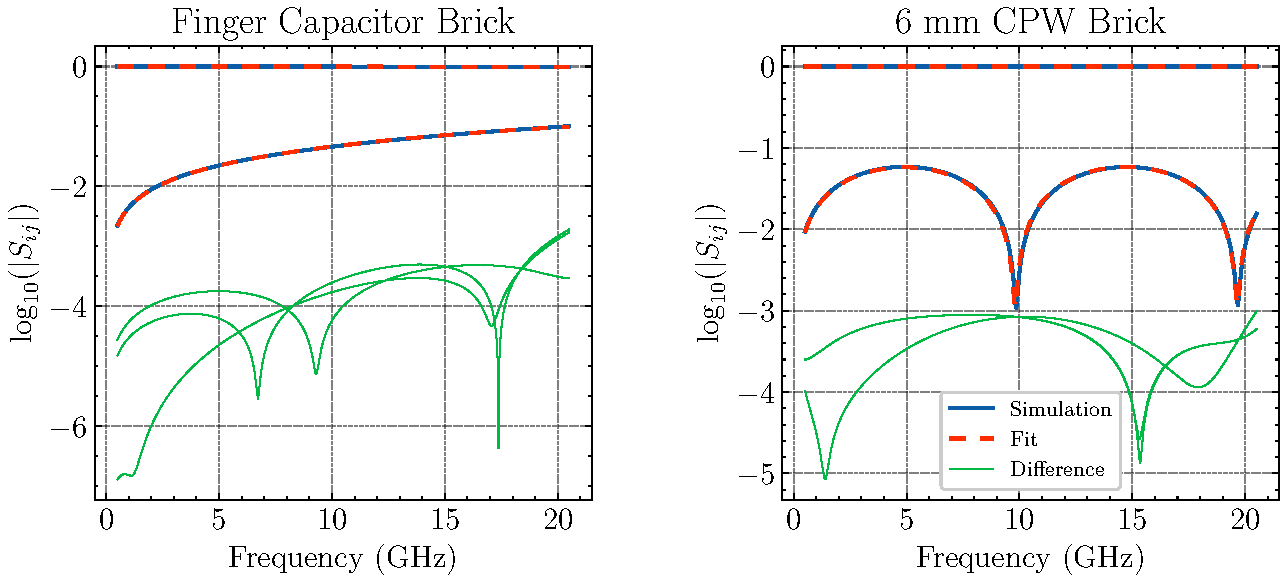
\includegraphics[width=\textwidth]{figures/cap_res_fit.pdf}
    \caption{Fitting results for the capacitor and CPW bricks shown in Fig.\ \ref{fig:cap_res_cap_split}. After converting the fitted rational impedance function to S-parameters, it is compared to the S-parameters from the simulation. All the S-parameters and differences are plotted on the same plot.}
    \label{fig:cap_res_fit}
\end{figure}

\begin{figure}[!h]
    \centering
    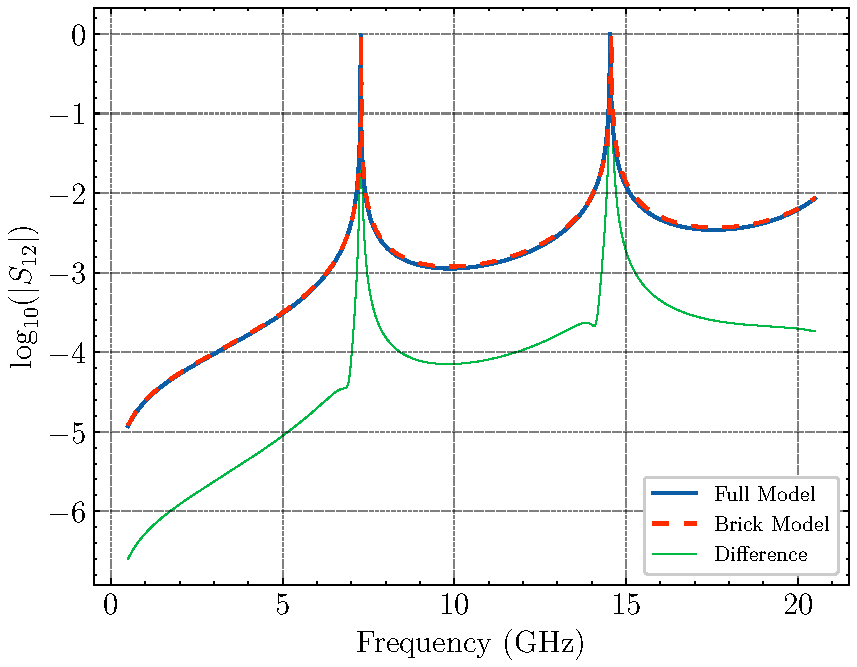
\includegraphics[width=0.6\textwidth]{figures/full_vs_brick.pdf}
    \caption{Difference between the $S_{12}$ parameter from the simulation of the full model in Fig.\ \ref{fig:cap_res_cap_full} and the interconnected brick model in Fig.\ \ref{fig:cap_res_cap_split}.}
    \label{fig:full_vs_brick}
\end{figure}

\begin{figure}[!h]
    \centering
    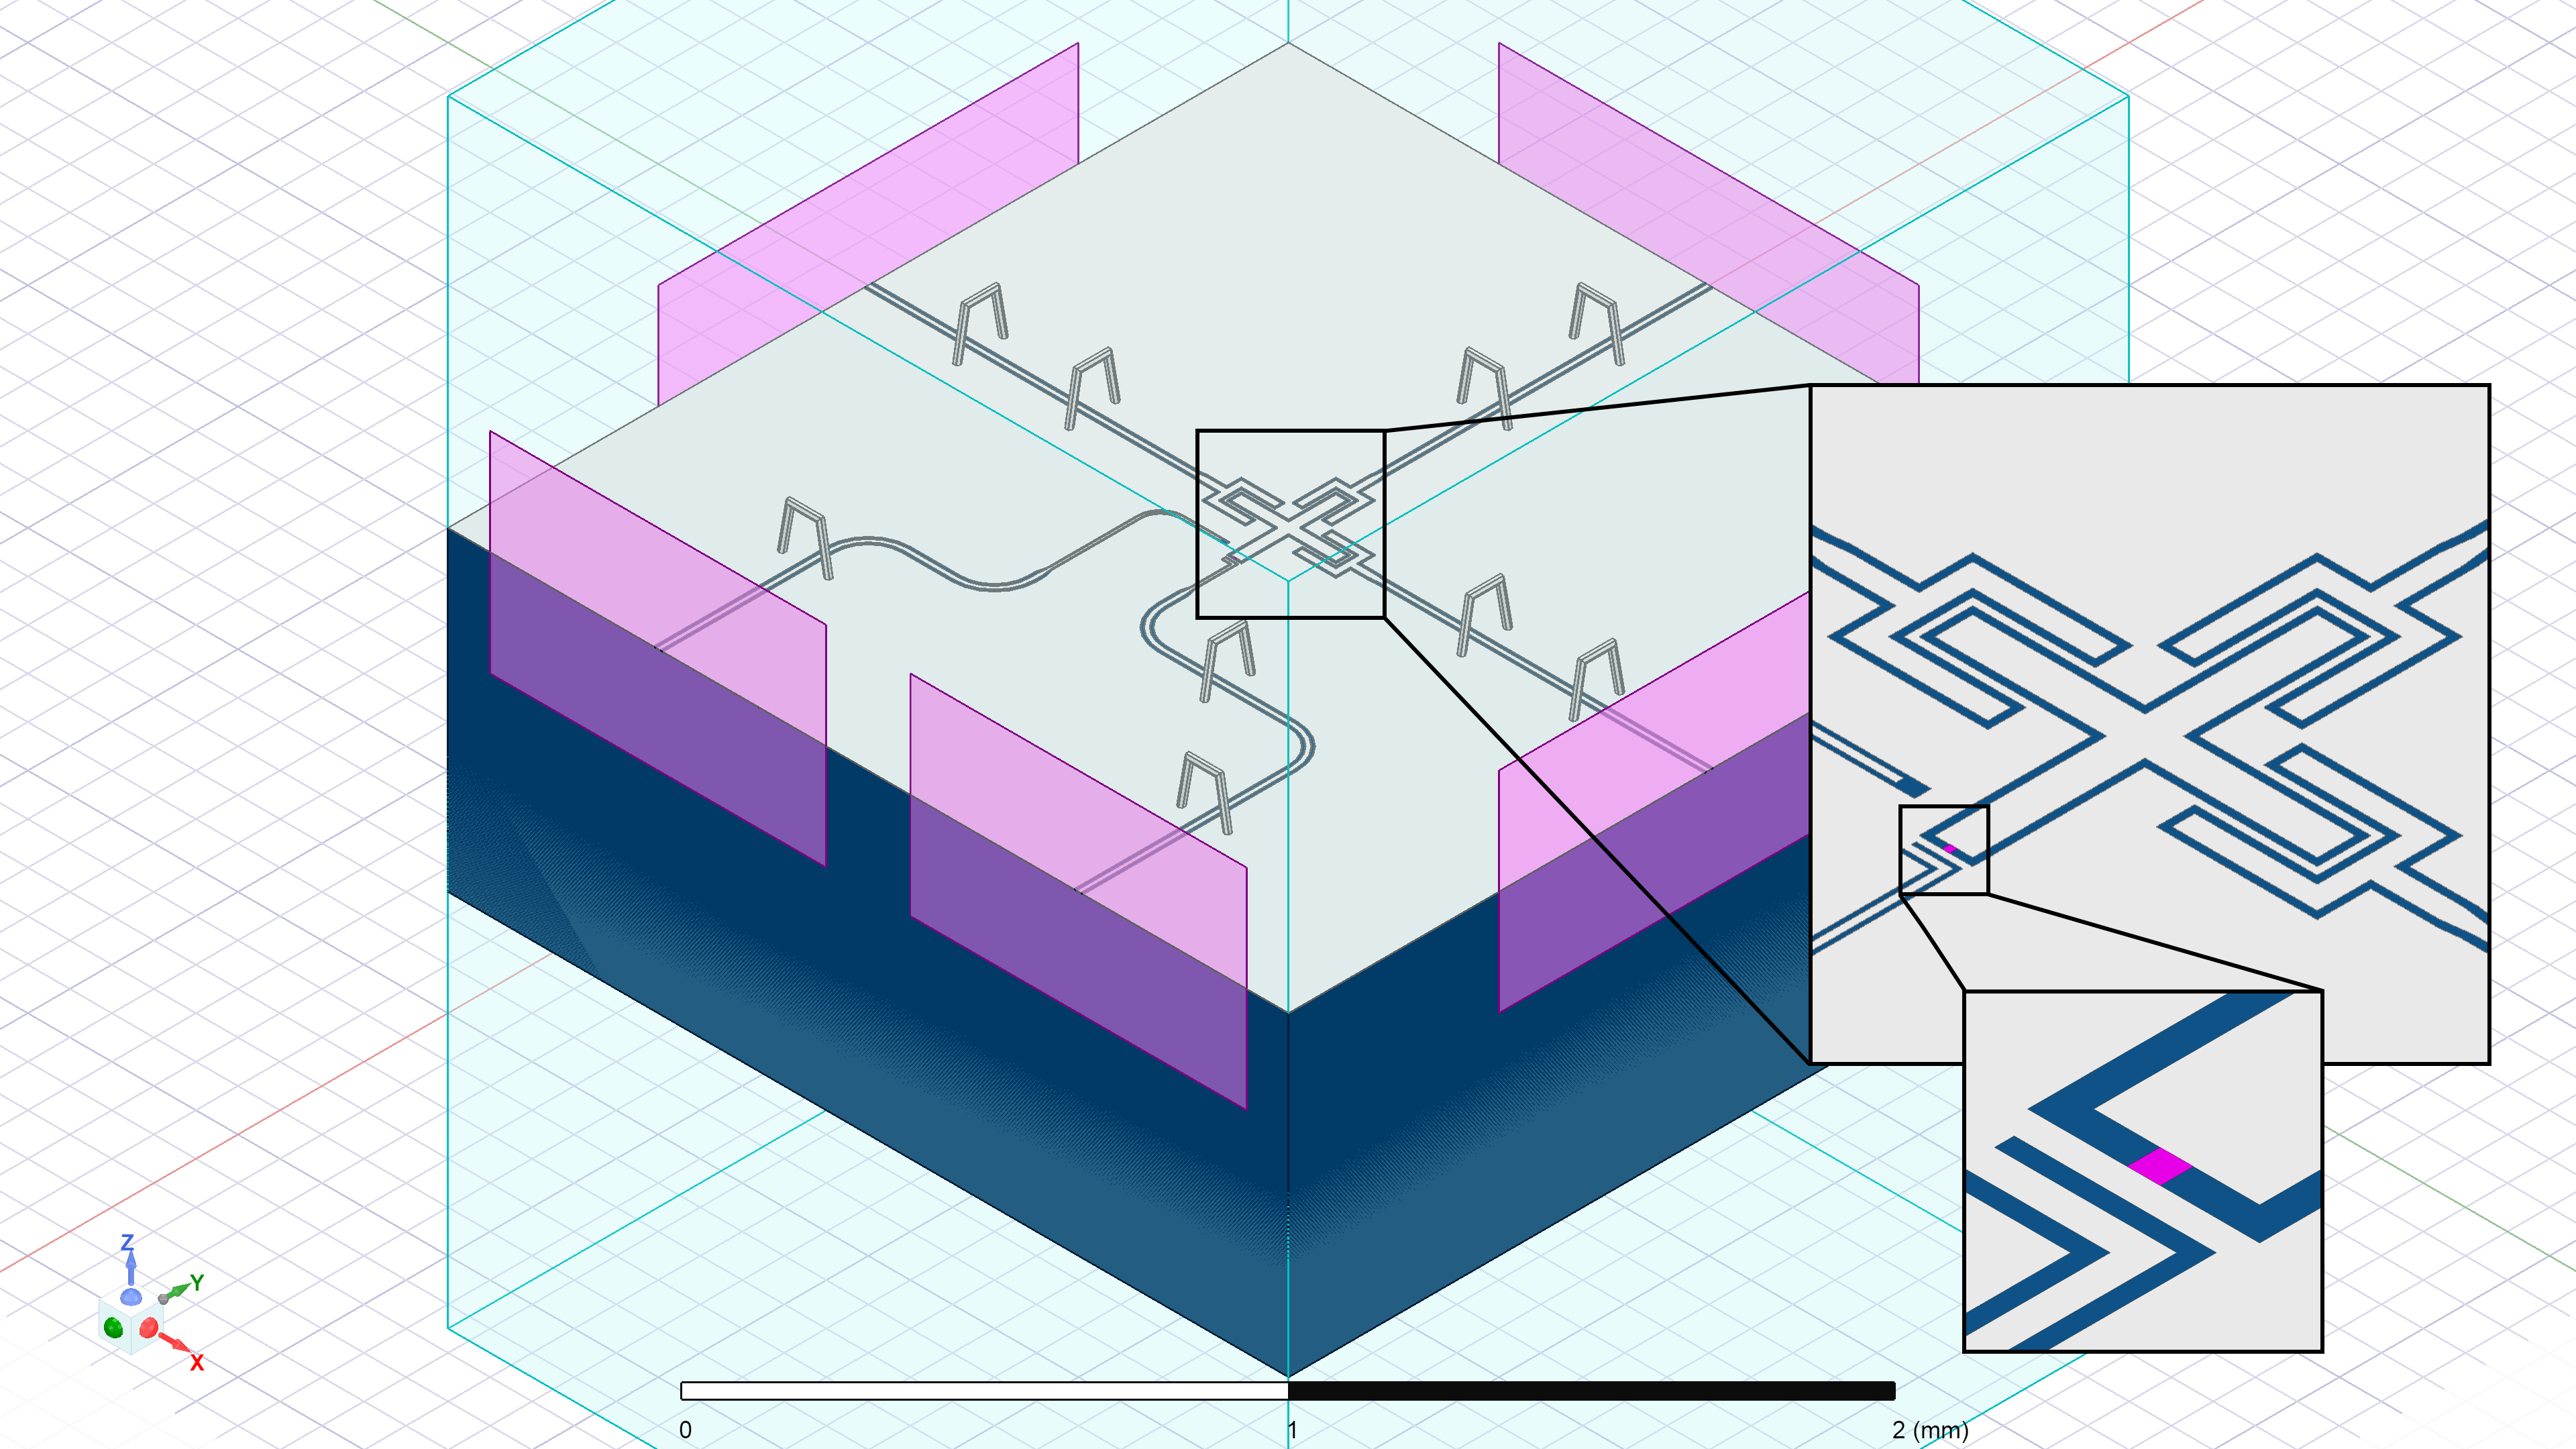
\includegraphics[width=\textwidth]{figures/xmon_extra_zoom.png}
    \caption{Brick model containing an Xmon style qubit \cite{xmon}. On the lower side of the cross, a lumped port (purple) is in the position where the SQUID would be located. Of the five wave ports on the boundary of the model, four correspond to CPW lines that are capacitively coupled to the qubit. The fifth wave port corresponds to a flux control line.}
    \label{fig:xmon_brick}
\end{figure}

Next, we look at a brick simulation that contains a transmon qubit. For qubits, we will have a lumped port that is located inside the boundaries of the simulation, unlike the wave ports previously seen. This lumped port is precisely the Josephson junction or ``qubit'' port that has been discussed in previous sections. The specific model we will discuss now is shown in Fig.\ \ref{fig:xmon_brick}. We want to use this model to discuss some more details that must be considered during the fitting process. When it comes to fitting this model, we need to be careful when dealing with the flux line port. Because the flux line is galvanically connected to the ground plane, it can be difficult to obtain a rational approximation of the form \ref{eq:impedance} with a positive definite DC residue. This is because the flux port components of the DC residue would be zero for a network like this. The fitting process can get close by including very small residue components and high frequency resonant modes, but this can cause unwanted effects in the Hamiltonian. To avoid these issues, we can fit the simulated impedance when the flux port is left open, and use this result when interconnecting with other bricks and constructing a Hamiltonian. However, we can still use the fit that includes the flux port for decay rate estimation. The results for fitting the simulated impedance for the model in Fig.\ \ref{fig:xmon_brick} are shown in Fig.\ \ref{fig:xmon_fit}. The fit including the flux line port struggles at low frequency due to the difficulty of attempting to fit the small residues and it also requires a number of poles outside of the visible frequency range. We would like to avoid including these types of poles when possible. When the flux port is left open, the fit for the remaining ports only requires one degenerate pole far out in the frequency range. We have found that allowing for a single degenerate pole when working with the electromagnetic models is sometimes needed for the fits to be accurate and this does not cause problems with the Hamiltonians. Sometimes, these degenerate poles and their residues can be thought of as an approximation to the infinite frequency pole that we have left out of (\ref{eq:impedance}).
\begin{figure}[!t]
    \centering
    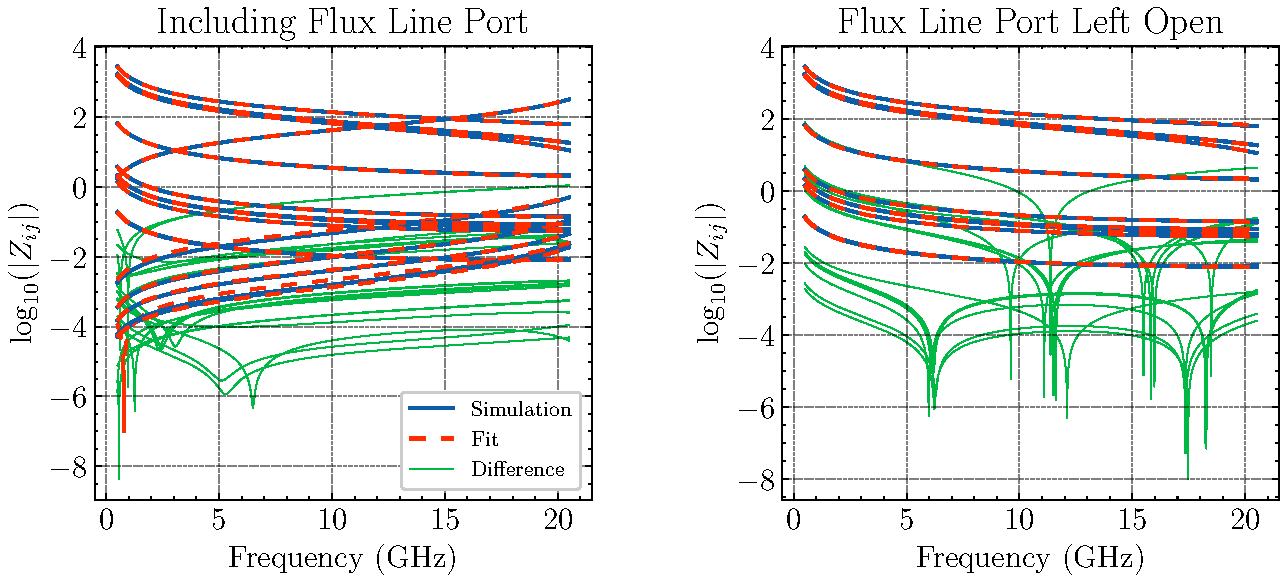
\includegraphics[width=\textwidth]{figures/xmon_fit.pdf}
    \caption{Impedance fit results for the simulation of the model shown in Fig.\ \ref{fig:xmon_brick}. On the left, the impedance including the flux line port is fitted. Note that the curves going to zero at low frequency on the left correspond to the parameters involving the flux line. In the fit on the right, the flux line port is left open to avoid inaccuracies brought in by trying to fit for the small residues corresponding to the flux line. All impedance parameters and differences between the fit and simulation are plotted together.}
    \label{fig:xmon_fit}
\end{figure}

When leaving the flux port open, we can obtain the Maxwell capacitance matrix that corresponds to the ports by inverting the DC residue. We then compare this to a Maxwell capacitance matrix obtained from a simulation in Ansys Q3D \cite{ansys_q3d}. In the Q3D simulation, the capacitance is computed between the metallic islands corresponding to the cross forming the Xmon and the CPWs leading to the boundary of the model. These matrices and differences are given in Appendix \ref{appendix:q3d_vs_hfss}. The differences are largest for the coupling capacitances that are small ($<$ 1 fF). Otherwise, estimates of the capacitance from fitting the HFSS model don't differ by more than 7\%. This difference is not caused by the fitting, and additional HFSS simulations and fits restricted to a low frequency range of 100 MHz to 1 GHz yield similar results. The differences likely come from the fact that the two simulation methods are different (HFSS is full-wave and Q3D is quasi-static) in addition to the different meshes and different port definitions in both models. There is the possibility to use Q3D within the HFSS simulation to solve the DC point, but with the combination of wave and lumped ports used in our models, this option is not available. For our examples here, we will use the models from HFSS, but it should be noted that improvements for the estimation at the DC point should be explored in the future within Ansys and potentially other simulation software.

\newpage

Taking a collection of bricks and their corresponding rational impedance functions, we can interconnect them to make a larger model. As an example, we consider the model in Fig.\ \ref{fig:triple_xmon}. In this model there are three resonator-coupled Xmon qubits. Each Xmon is also coupled to its own readout resonator that is also coupled to a common readout line. By looking at the S-parameters for this network, we clearly see which resonant modes couple the qubits to each other and to the feedline. Some of the relevant S-parameters are shown in Fig.\ \ref{fig:triple_xmon_S}.

\begin{figure}[h!]
    \centering
    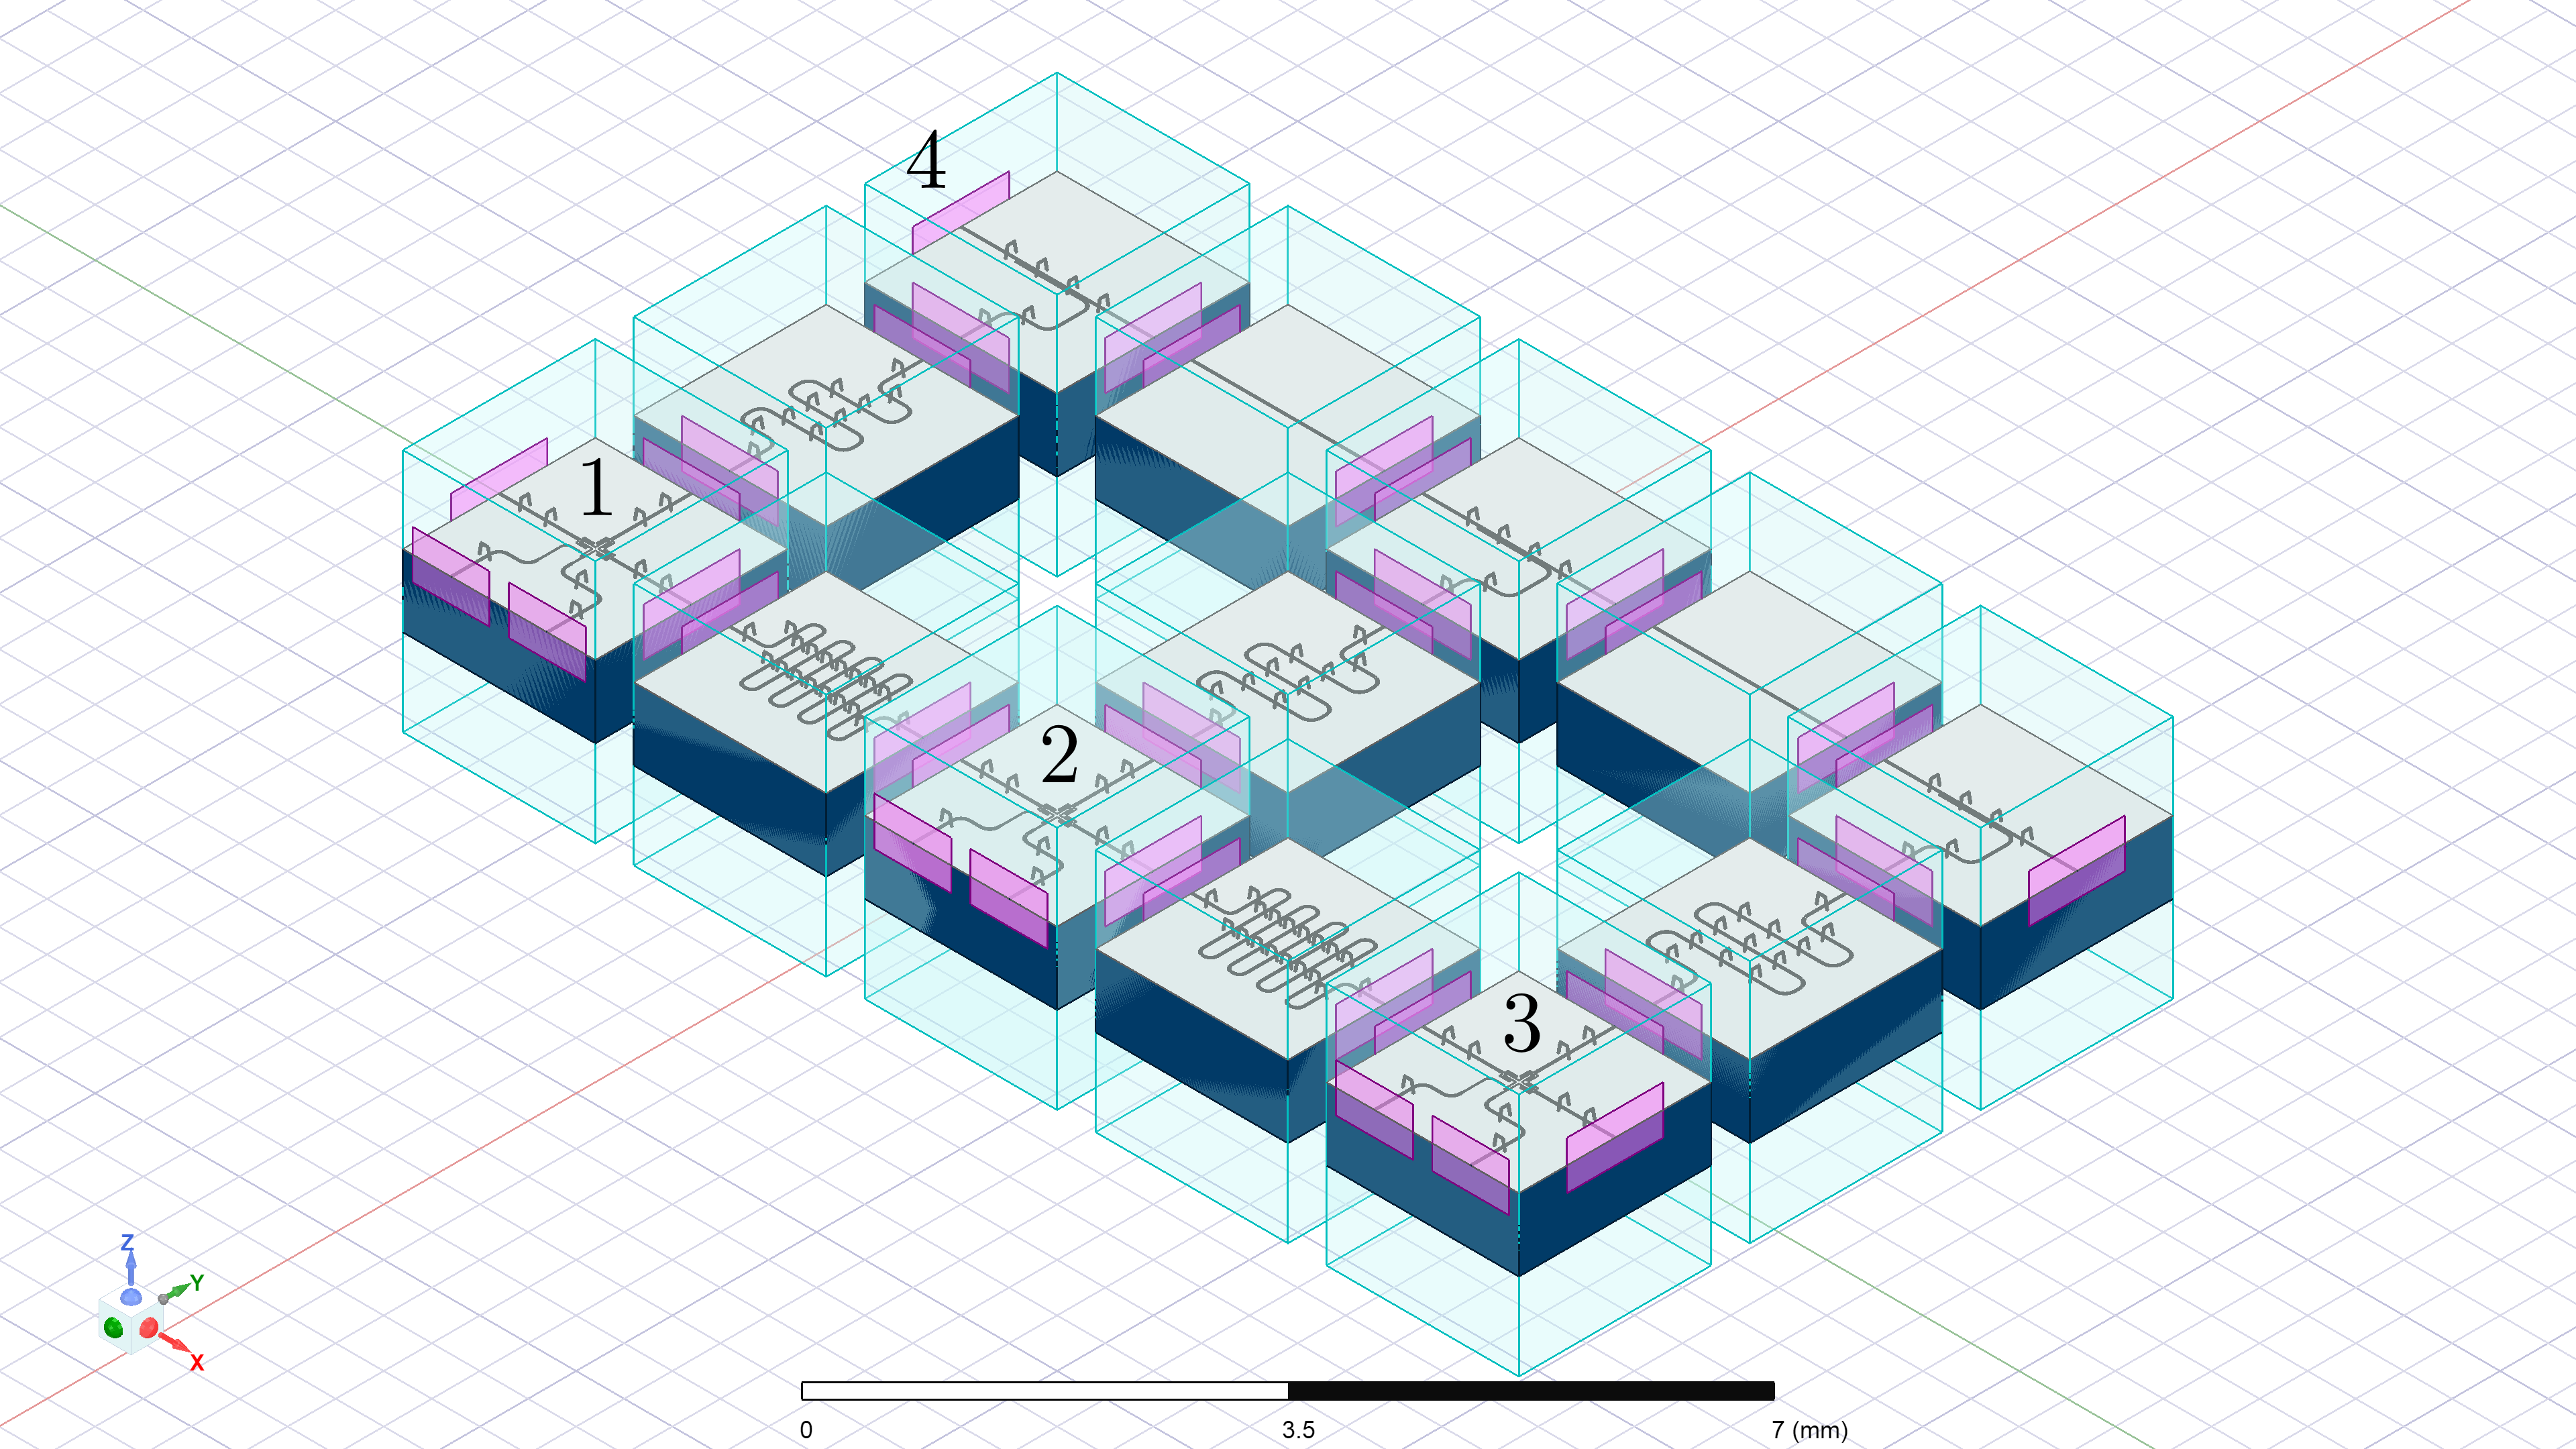
\includegraphics[width=\textwidth]{figures/triple_qubit_labeled.png}
    \caption{Brick model of a three Xmon circuit. The qubits are coupled to each other through half-wave resonators. Each qubit is also capacitively coupled to its own half-wave readout resonator that is capacitively coupled to a common readout line.}
    \label{fig:triple_xmon}
\end{figure}

\begin{figure}[h!]
    \centering
    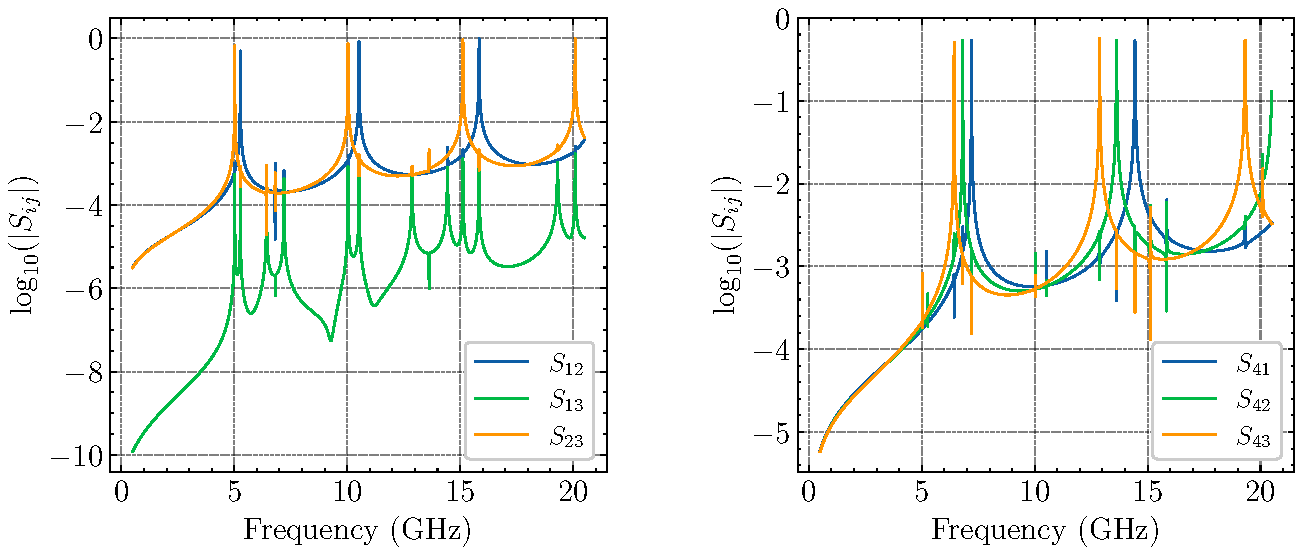
\includegraphics[width=\textwidth]{figures/three_qubit_S.pdf}
    \caption{Some of the matrix elements of the S-parameter for the fully interconnected network shown in Fig.\ \ref{fig:triple_xmon}. Port numbers are shown in Fig.\ \ref{fig:triple_xmon}. Ports 1-3 correspond to the three qubit junction ports. Port 4 corresponds to the left port of the feedline in Fig.\ \ref{fig:triple_xmon}.}
    \label{fig:triple_xmon_S}
\end{figure}

\newpage

With the rational impedance function corresponding to the fully interconnected model in Fig.\ \ref{fig:triple_xmon}, we can also build a circuit Hamiltonian of the form (\ref{eq:transmon_resonator_ham}). This can then be used to estimate the effective coupling rates between the qubits using (\ref{eq:eff_qubit_coupling}). We can also estimate the dispersive shift in the fundamental resonance frequency of each readout resonator using (\ref{eq:dispersive_shifts}). For the circuit in Fig.\ \ref{fig:triple_xmon}, these effective coupling rates and dispersive shifts are shown in Fig.\ \ref{fig:triple_xmon_geff_chi}. Additionally, with the fully interconnected model, we can estimate the relaxation times for each qubit by using (\ref{eq:matrix_eoms}) or (\ref{eq:qubit_decay_admittance}). The results for our example circuit in Fig.\ \ref{fig:triple_xmon} are shown in Fig.\ \ref{fig:triple_xmon_T1}.

\begin{figure}[h!]
    \centering
    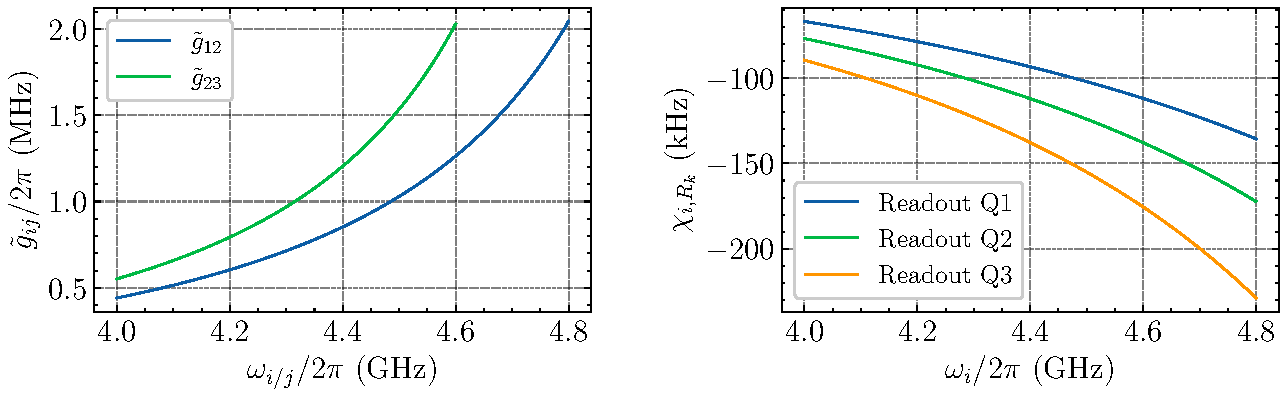
\includegraphics[width=\textwidth]{figures/three_qubit_geff_chi.pdf}
    \caption{Effective qubit coupling rates and readout resonator dispersive shifts for the interconnected model of Fig.\ \ref{fig:triple_xmon}. Left: Effective coupling rates between the qubits (third qubit is fixed at 4 GHz while the other two qubit frequencies are varied). The fundamental frequencies for the coupling resonators are 5.268 GHz ($Q1 \leftrightarrow Q2$) and 5.023 GHz ($Q2 \leftrightarrow Q3$). A cutoff frequency of 21.5 GHz is used for this example to avoid incorrect predictions of resonant modes outside the fitting range. Right: The dispersive shift in the fundamental modes of the readout resonators. The fundamental frequencies of the readout resonators for qubits 1 to 3 are 7.205 GHz, 6.812 GHz, and 6.435 GHz, respectively.}
    \label{fig:triple_xmon_geff_chi}
\end{figure}

\begin{figure}[h!]
    \centering
    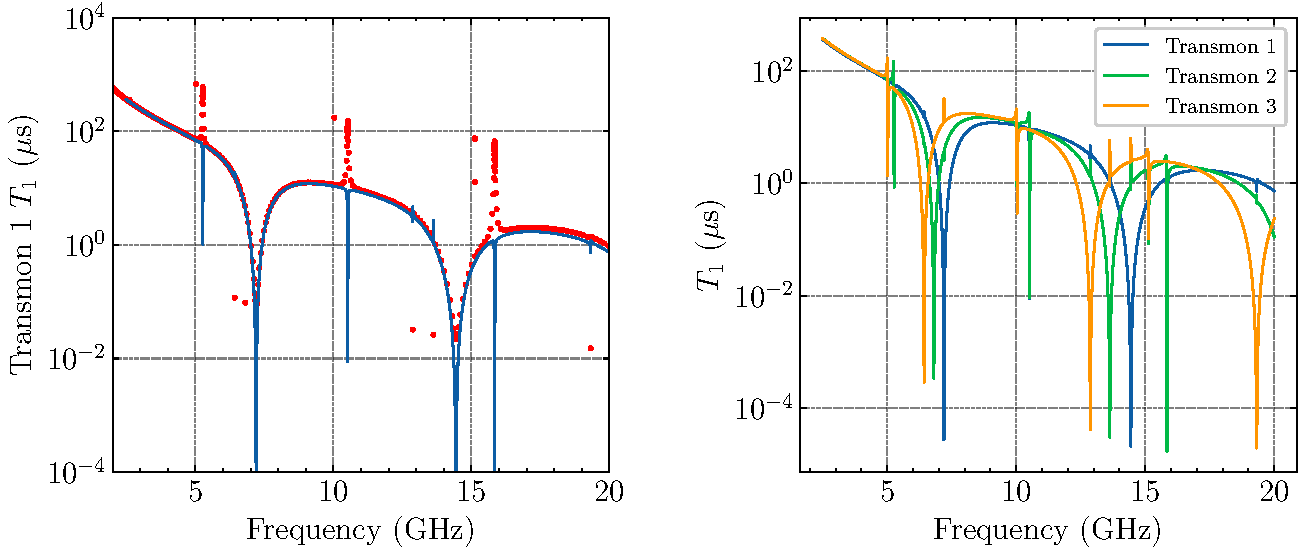
\includegraphics[width=\textwidth]{figures/three_qubit_T1.pdf}
    \caption{Relaxation times for the qubits in the circuit of Fig.\ \ref{fig:triple_xmon}. On the left plot, we focus only on qubit 1. For a sweep of the shunt inductance of qubit 1, the complex frequencies from (\ref{eq:matrix_eoms}) are plotted as red points. Isolated red points belong to the resonant modes that have a nearly fixed decay rate due to their small coupling to qubit 1. The blue line is the result of using (\ref{eq:qubit_decay_admittance}) with resistors shunting the external ports and no inductances shunting the qubit ports. On the right, we see the result from (\ref{eq:qubit_decay_admittance}) for all three qubits in the circuit.}
    \label{fig:triple_xmon_T1}
\end{figure}

Using these brick models, we can also estimate how the effective coupling through resonant modes present in a circuit will scale for multi-qubit devices. To do this, we recreate a qubit grid circuit similar to an example from \cite{solgun_sirf} where lumped elements were used. In our case, we use various bricks that correspond to electromagnetic models to create a grid of qubits. The circuit we consider is shown in Fig.\ \ref{fig:2x6}.

\begin{figure}[h!]
    \centering
    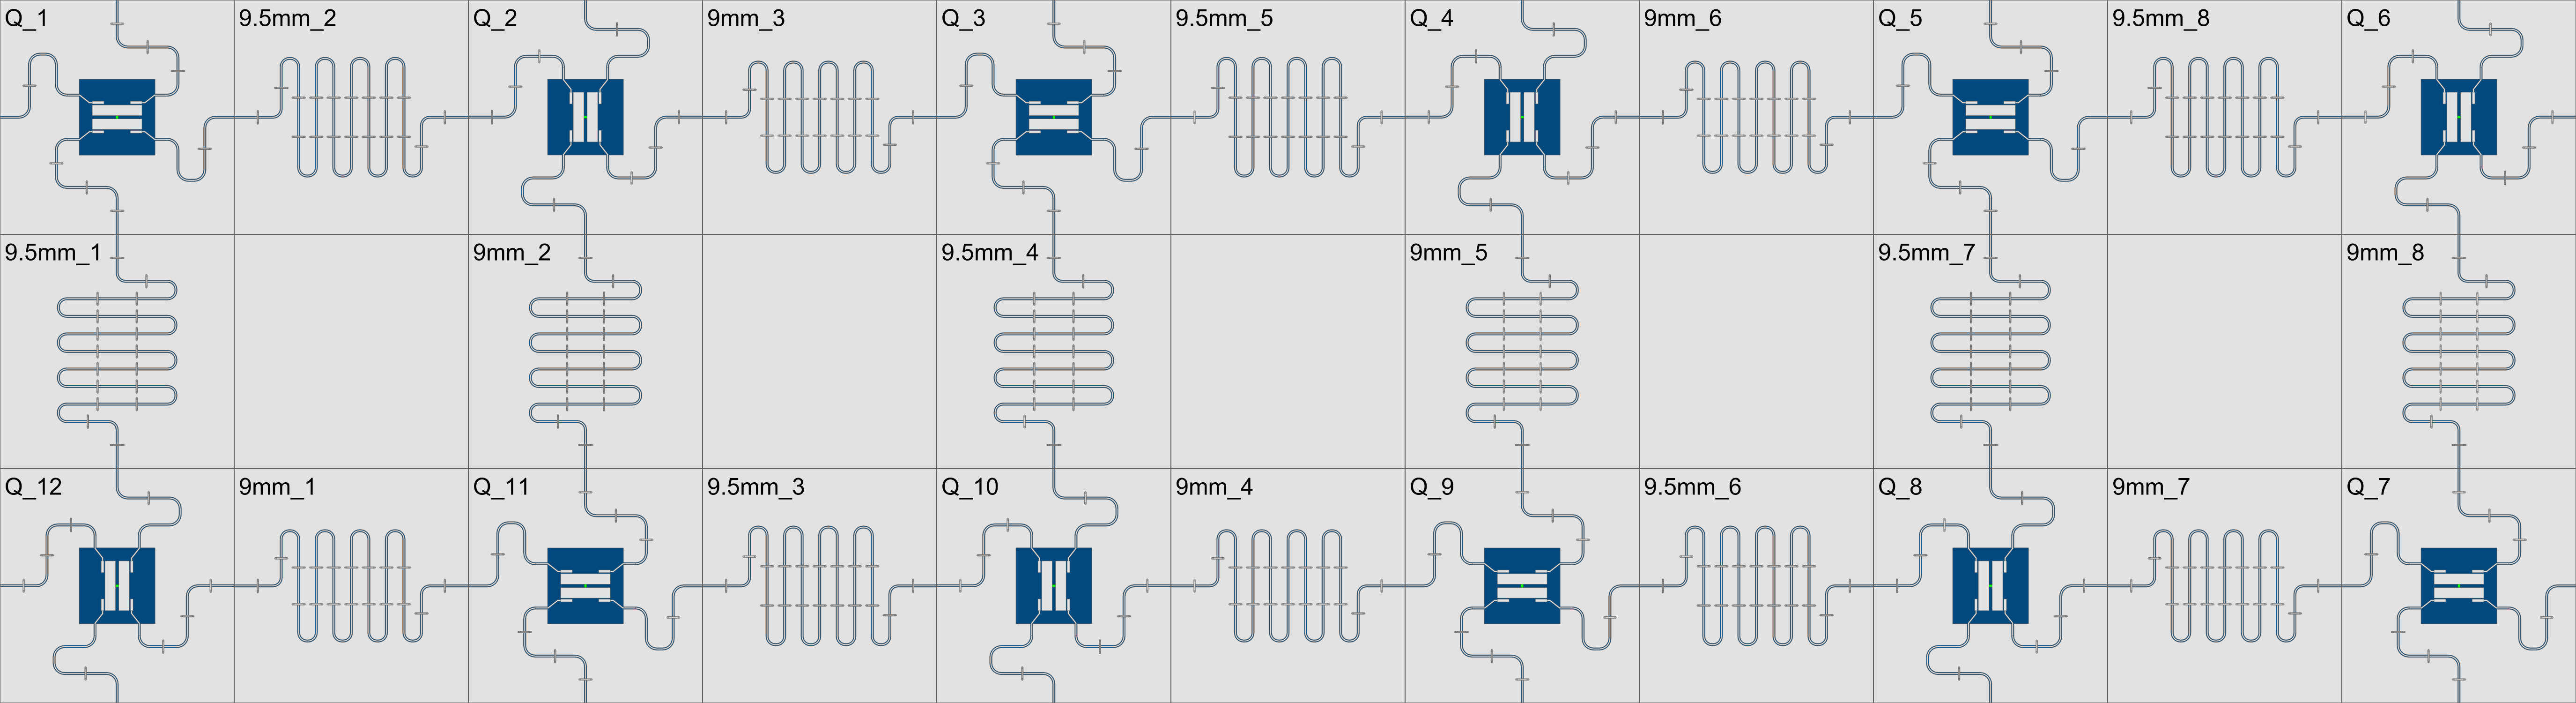
\includegraphics[width=\textwidth]{figures/2x6.png}
    \caption{A grid of IBM style transmons \cite{solgun_sirf} that are coupled through bus resonators. The qubits are numbered 1 to 12 starting from the top left and moving clockwise around the lattice.}
    \label{fig:2x6}
\end{figure}

After building the model of the circuit in Fig.\ \ref{fig:2x6}, we can compute the effective coupling rates between the qubits using (\ref{eq:eff_qubit_coupling}). The effective coupling of qubit 1 to all of the other qubits is shown in Fig.\ \ref{fig:2x6_coupling}. In this figure, we can see the exponential decay of the effective coupling as we get further from qubit 1. This exponential decay was also found for networks of this type in the lumped element example of \cite{solgun_sirf}. It is also expected for networks of this form if the direct capacitive coupling is excluded (see Appendix \ref{appendix:banded_cap}).

\begin{figure}[h!]
    \centering
    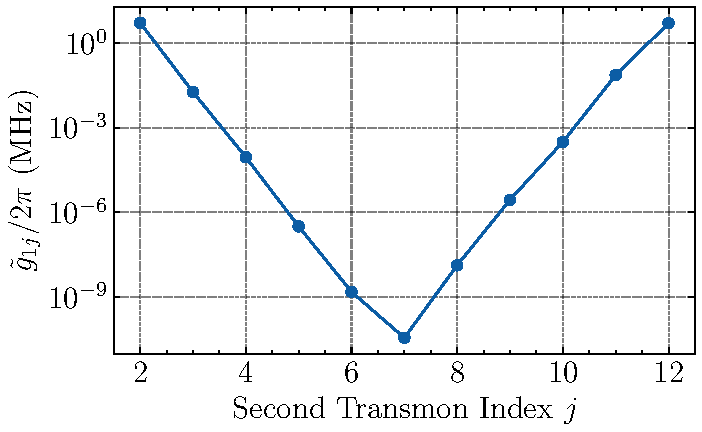
\includegraphics[width=0.5\textwidth]{figures/2x6_coupling.pdf}
    \caption{Effective coupling of qubit 1 of the circuit in Fig.\ \ref{fig:2x6} to all of the other qubits. All qubits are frequencies are fixed at 4.25 GHz. In practice, we would not see the influence of such small coupling rates $g/2\pi \lesssim 1$ kHz, but this can still be a useful tool for verifying that the long range coupling through resonant modes in a specific layout is negligible.}
    \label{fig:2x6_coupling}
\end{figure}

\subsection{Parasitic Resonances}
As the number of components present within superconducting circuits increases, we may start to see parasitic resonances at frequencies closer to the operating frequency range of the qubits. These parasitic resonances at lower frequencies could have a non-negligible impact on the effective coupling between qubits. Depending on where these resonant modes arise (physically and in frequency), it is be useful to see how changes to device geometry results in changes of the couplings to these parasitic resonances.

As an example, we consider a parasitic resonance that is present within a chain of Xmons. The parasitic resonance we will be concerned with is the lowest resonant mode of the chain structure that is above the operating frequencies of the qubits (around 4 to 6 GHz). Of course, there will be higher frequency parasitic resonances, but here we only consider the lowest as it should be the mode that contributes the most to any changes in effective coupling. In Fig.\ \ref{fig:xmon_1x3_eig}, we can see the electric field profile of the lowest resonant mode in a chain of three Xmons. The field profile and resonance frequency are found using the eigenmode solver within HFSS. While not super clear with just three Xmons, the outer two crosses participate less in the resonance than the center cross. This is clearer if we increase the length of the chain as shown in Fig.\ \ref{fig:xmon_1x10_eig}. We can also see that when adding more Xmons to the chain, the frequency of the parasitic resonance in the chain decreases. Using the eigenmode solver in HFSS, we obtain the results in Fig.\ \ref{fig:xmon_chain_res} that show how the frequency of the resonance decreases as we increase the number of Xmons.
\begin{figure}[h!]
    \centering
    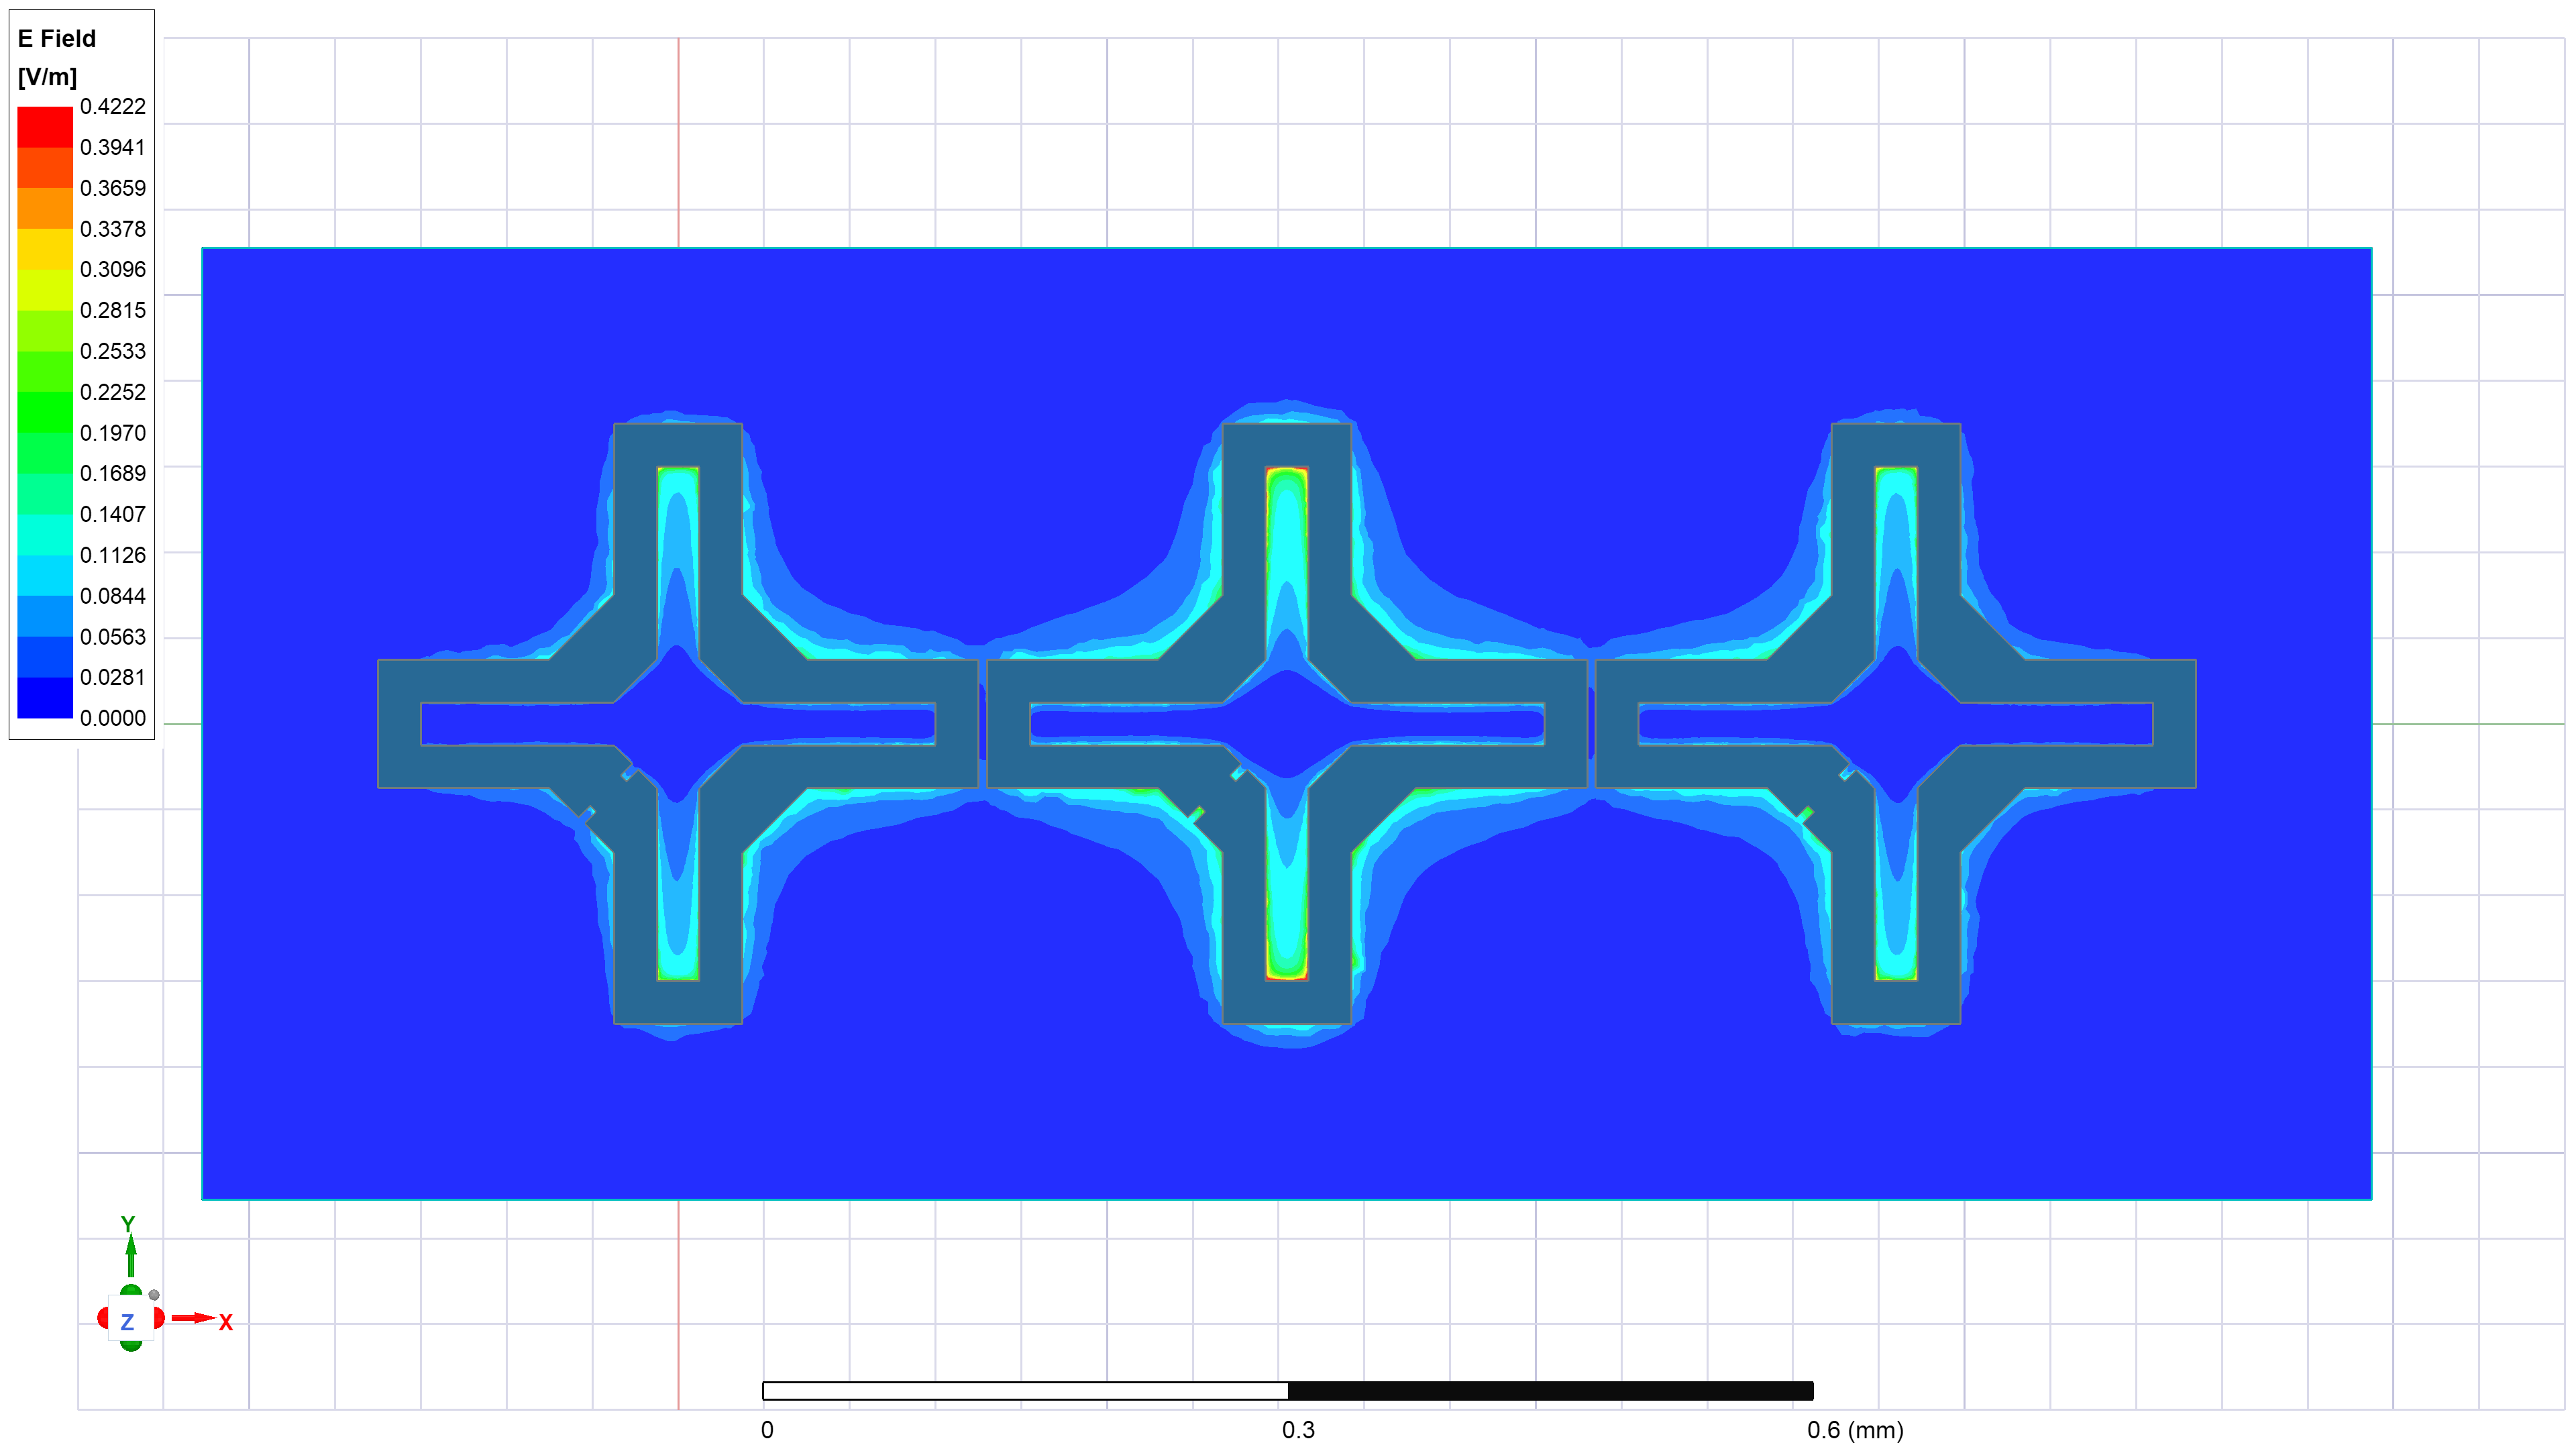
\includegraphics[width=0.75\textwidth]{figures/xmon_1x3_eig.png}
    \caption{Magnitude of the electric field at the surface of the perfect conductor in a three Xmon chain. This is the lowest resonant mode above the operating range of the qubits. The resonant frequency is 52.5322 GHz.}
    \label{fig:xmon_1x3_eig}
\end{figure}

\begin{figure}[h!]
    \centering
    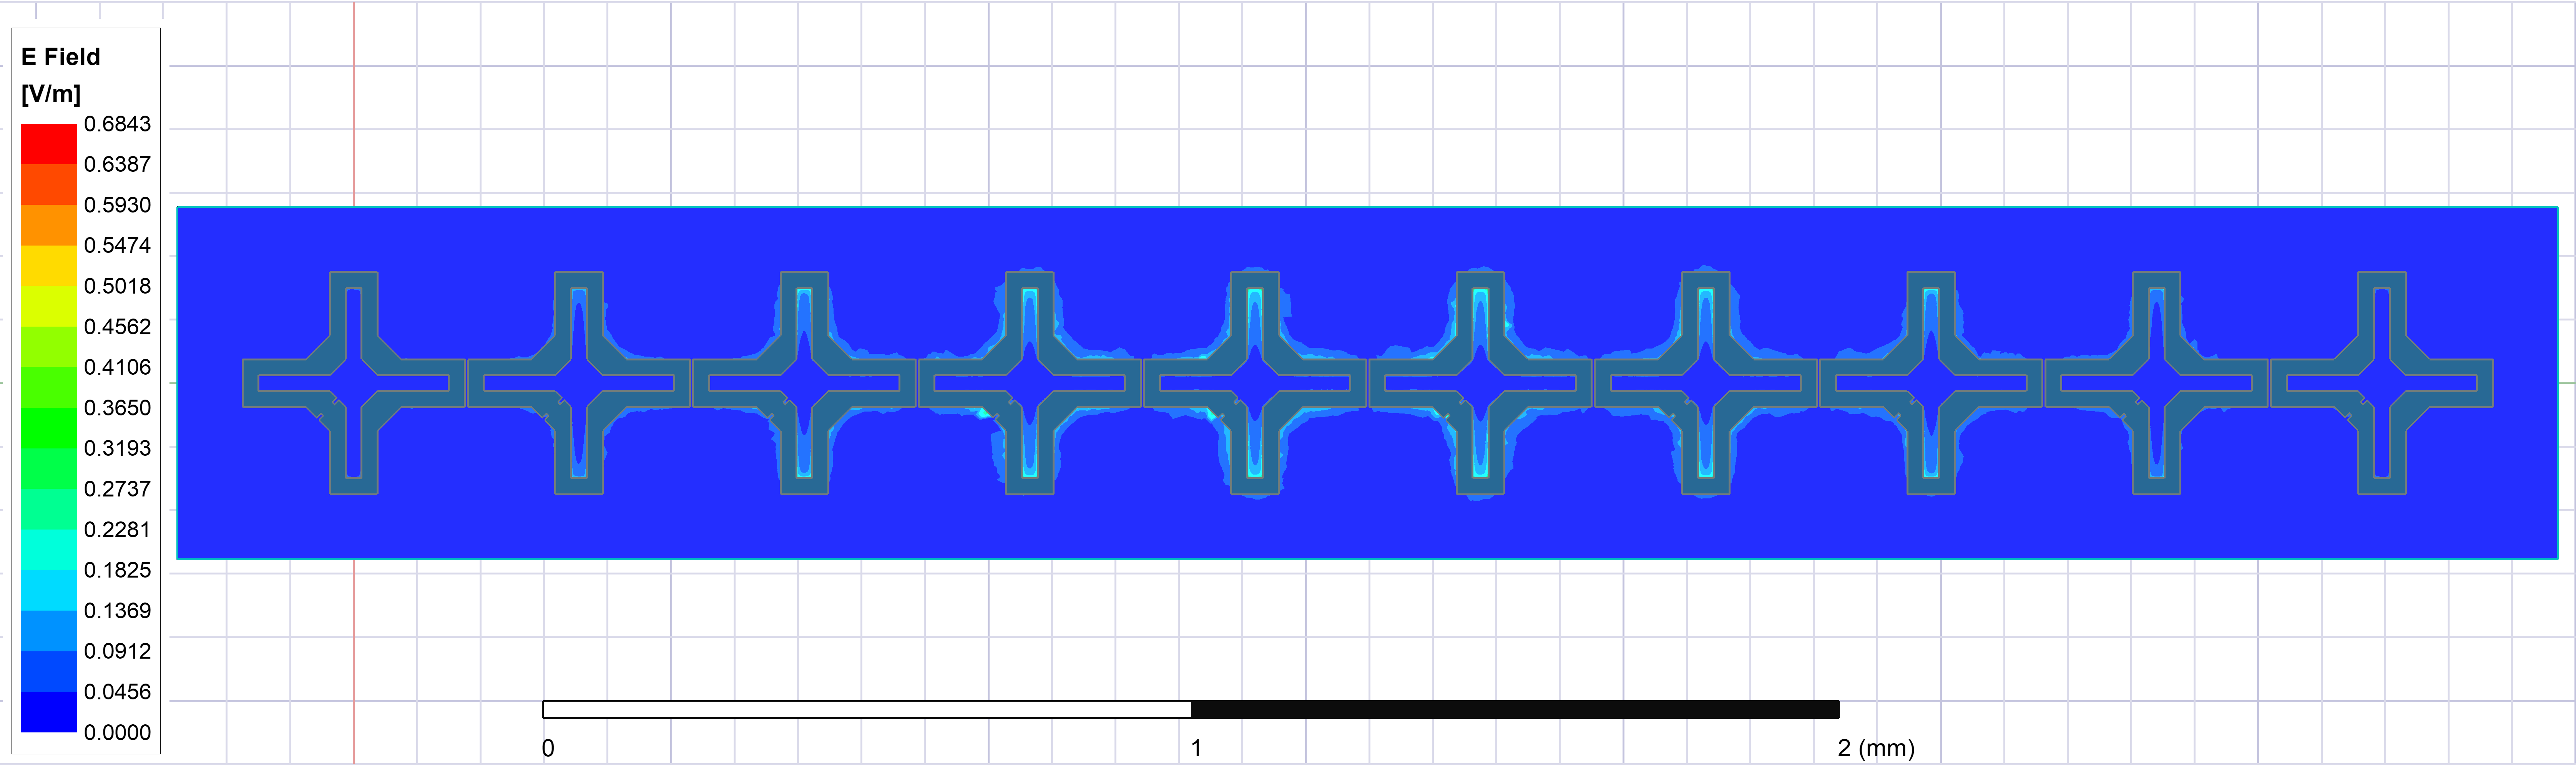
\includegraphics[width=\textwidth]{figures/xmon_1x10_eig.png}
    \caption{Magnitude of the electric field in a ten Xmon chain for the lowest resonant mode of 37.8159 GHz in the structure.}
    \label{fig:xmon_1x10_eig}
\end{figure}

To estimate the coupling rates of the qubits to this parasitic resonance, we can try to use the vector fitting methods of Section \ref{section:vector_fitting}. Including lumped ports at the positions of the junctions, we obtain the impedance parameter in HFSS over a broad frequency range (1 GHz to 80 GHz) so that the lower parasitic resonance is visible. Unfortunately, the traditional vector fitting struggles to give a good fit for the whole frequency range with the results shown in Fig.\ \ref{fig:xmon_3_4_fit}. Due to the poor fit, the estimated coupling rates are likely inaccurate. We can alternatively look at the S-parameters to understand how the qubits are coupled to the parasitic resonance relative to one another. This can also be used to track how coupling to parasitic resonances changes for different device geometry. In Fig.\ \ref{fig:xmon_3_4_S} we can see the diagonal matrix elements of the S-parameters for the three and four Xmon chains. This clearly shows which qubits are most strongly coupled to the parasitic resonance. If changes are made to the device, we can potentially track how the S-parameters compare between devices to see if the coupling of the qubits to these parasitic resonances has gone down. In Fig.\ \ref{fig:xmon_5_6_S} we show similar plots for the five and six Xmon chains.

\begin{figure}[h!]
    \centering
    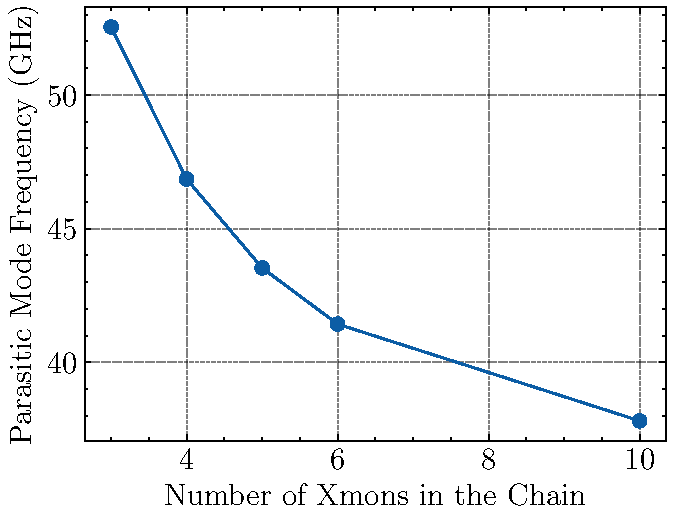
\includegraphics[width=0.5\textwidth]{figures/xmon_chain_res.pdf}
    \caption{Lowest parasitic resonance frequencies for different numbers of Xmons in a chain. Resonance frequencies are computed using the eigenmode solver within HFSS.}
    \label{fig:xmon_chain_res}
\end{figure}

\begin{figure}[h!]
    \centering
    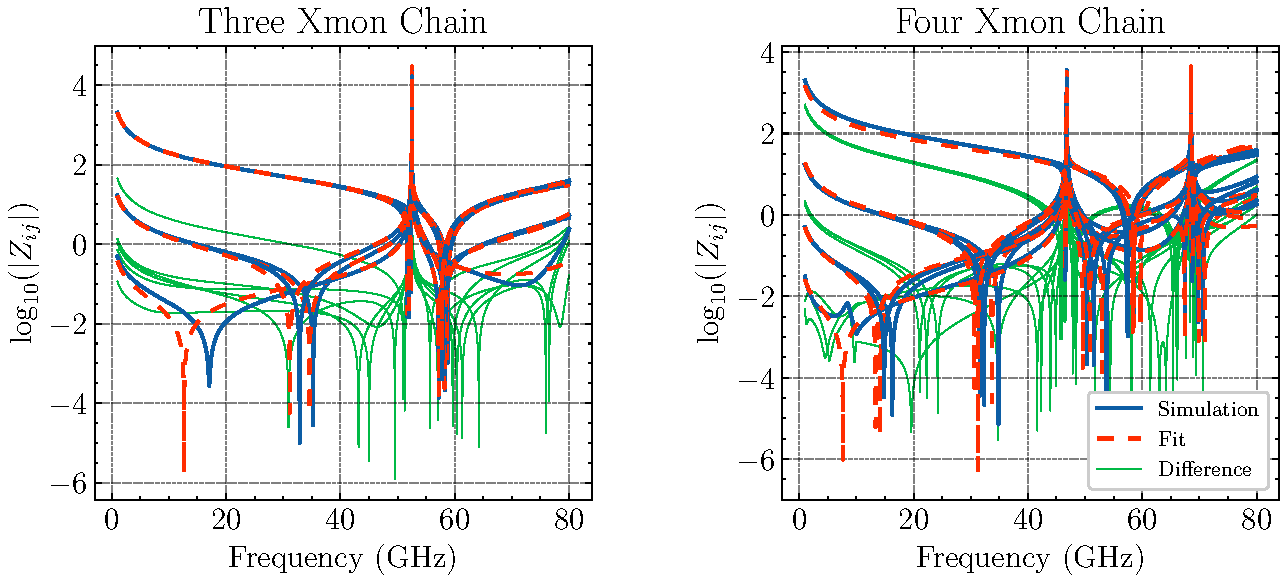
\includegraphics[width=\textwidth]{figures/xmon_chain_fitting.pdf}
    \caption{Attempts at fitting the impedance parameter for the three and four Xmon chains. For the three qubit chain shown in Fig.\ \ref{fig:xmon_1x3_eig}, we find that magnitudes of the coupling rates of the three qubits to the lowest parasitic resonance mode are 103, 228 and 167 MHz from left to right. For the four qubit chain, the magnitudes of the coupling rates are 129, 292, 321 and 204 MHz. This is for the qubit frequencies fixed at 4 GHz. The coupling rates are not symmetric due to the junction ports being off center on each cross. Due to the poor fitting of the DC and parasitic resonance residues, the coupling rates are likely inaccurate as we expect the coupling rates of the qubits to the resonance to be lower in the four Xmon chain (see Fig.\ \ref{fig:xmon_3_4_S}).}
    \label{fig:xmon_3_4_fit}
\end{figure}

\newpage

\begin{figure}[!ht]
    \centering
    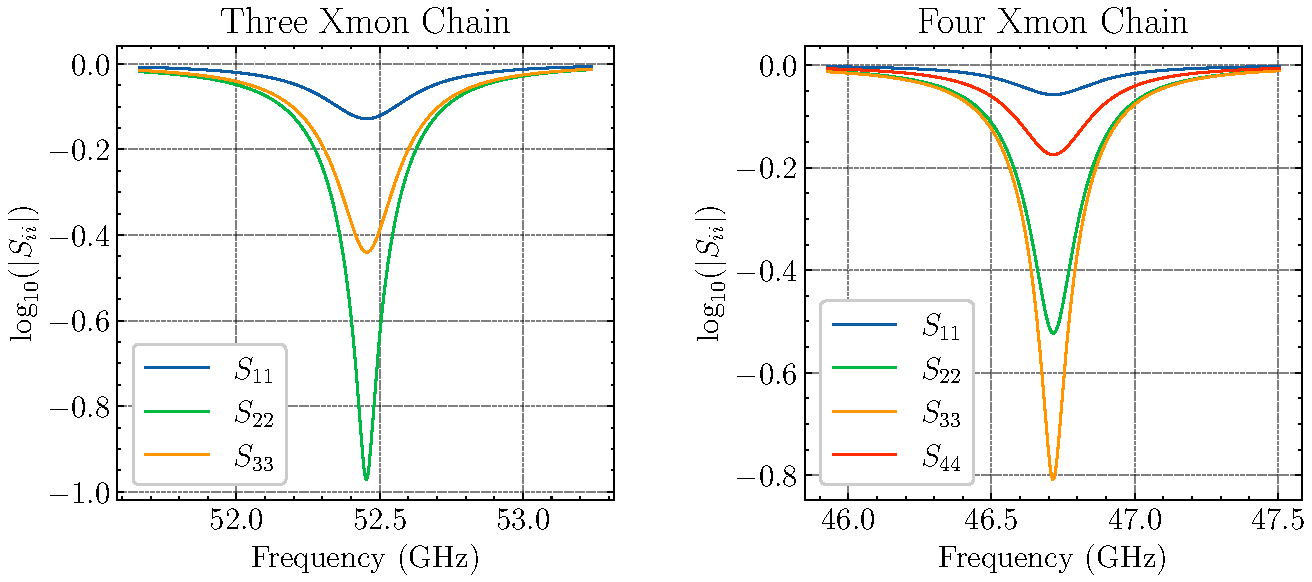
\includegraphics[width=\textwidth]{figures/xmon_chain_S.pdf}
    \caption{Diagonal matrix elements of the S-parameters for the three and four Xmon chains. The qubit ports are numbered left to right on the chain. We can see that closer to the center of the chain, the qubits are more strongly coupled to the parasitic resonance. Also, we can see that in the four Xmon chain, the qubits are coupled less to the parasitic resonance than in the three Xmon chain.}
    \label{fig:xmon_3_4_S}
\end{figure}

\begin{figure}[!ht]
    \centering
    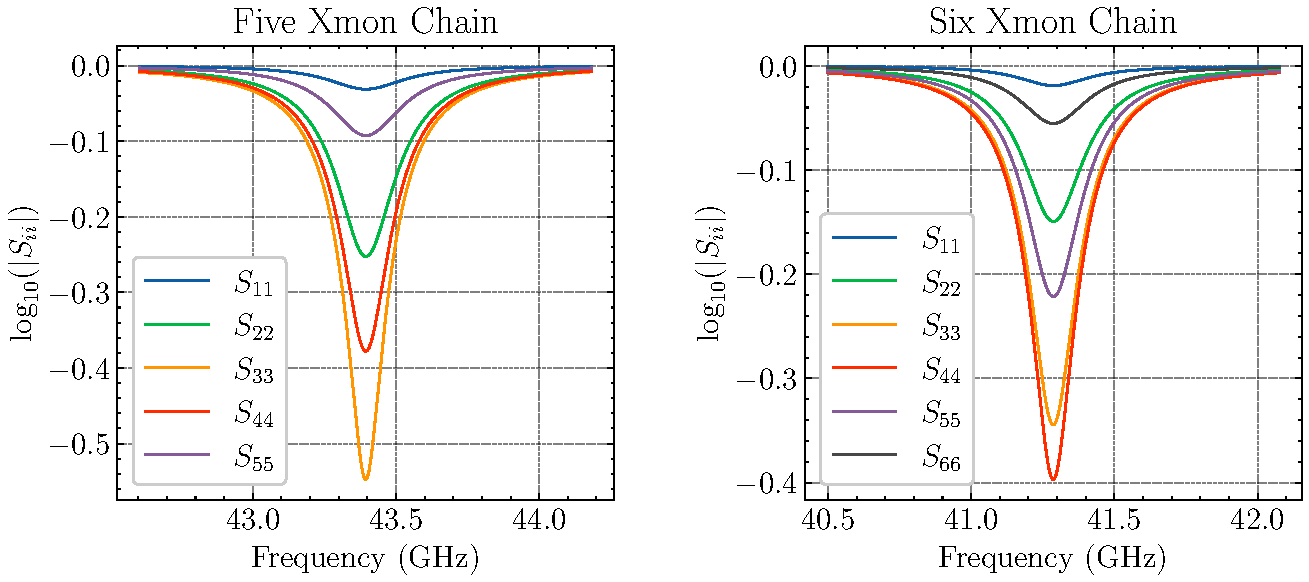
\includegraphics[width=\textwidth]{figures/xmon_chain_S_5_6.pdf}
    \caption{Similar to Fig.\ \ref{fig:xmon_3_4_S}, but for the five and six Xmon chains.}
    \label{fig:xmon_5_6_S}
\end{figure}
